\documentclass[10pt,twocolumn,letterpaper]{article}

\usepackage{iccv}
\usepackage{times}
\usepackage{epsfig}

\usepackage{graphicx}
\usepackage{tabularx}
\graphicspath{{figures/}}
\usepackage{makecell}
\usepackage{flushend}

\usepackage{amsmath}
\usepackage{amssymb}
\usepackage{color}
\usepackage{caption}
\usepackage{subcaption}
\usepackage{multirow}
\usepackage{bbm}


% \usepackage{titlesec}
\newcounter{example}%[section]
\renewcommand{\theexample}{\arabic{example}}
\newenvironment{example}{
        \vspace{1.5ex}
        \refstepcounter{example}
        {\noindent\bf Example \theexample:}}{
        \eop\vspace{1.5ex}}


\newcommand{\eat}[1]{}
\newcommand{\kw}[1]{{\ensuremath {\mathsf{#1}}}\xspace}
\newcommand{\eop}{\hspace*{\fill}\mbox{$\Box$}}
\newcommand{\kwlog}{\emph{w.l.o.g.}\xspace}
\newcommand{\stitle}[1]{\vspace{1.5ex}\noindent{\bf #1}}
\newcommand{\etitle}[1]{\vspace{0.8ex}\noindent{\underline{\em #1}}}
\newcommand{\aka}{\emph{a.k.a.}\xspace}
\newcommand{\gpmm}{\kw{GPM}}
\newcommand{\vqa}{\kw{VQA}}
\newcommand{\nlq}{Q_{nl}}
\newcommand{\eag}{G_{EA}}


% Include other packages here, before hyperref.

% If you comment hyperref and then uncomment it, you should delete
% egpaper.aux before re-running latex.  (Or just hit 'q' on the first latex
% run, let it finish, and you should be clear).
\usepackage[pagebackref=true,breaklinks=true,letterpaper=true,colorlinks,bookmarks=false]{hyperref}
\usepackage[capitalise]{cleveref}
%\Crefname{equation}{Eq.}{Eqs.}
%\Crefname{figure}{Fig.}{Figs.}
\Crefname{table}{Tab.}{Tabs.}
% \iccvfinalcopy % *** Uncomment this line for the final submission

\def\iccvPaperID{954} % *** Enter the ICCV Paper ID here
\def\httilde{\mbox{\tt\raisebox{-.5ex}{\symbol{126}}}}

% Pages are numbered in submission mode, and unnumbered in camera-ready
\ificcvfinal\pagestyle{empty}\fi
\begin{document}

%%%%%%%%% TITLE
\title{Visual Question Answering with Question Understanding and Reasoning}

\author{First Author\\
Institution1\\
Institution1 address\\
{\tt\small firstauthor@i1.org}
% For a paper whose authors are all at the same institution,
% omit the following lines up until the closing ``}''.
% Additional authors and addresses can be added with ``\and'',
% just like the second author.
% To save space, use either the email address or home page, not both
\and
Second Author\\
Institution2\\
First line of institution2 address\\
{\tt\small secondauthor@i2.org}
}

\maketitle
%\thispagestyle{empty}


%%%%%%%%% ABSTRACT
\begin{abstract}
Traditional techniques for visual question answering (\vqa) are mostly end-to-end neural network based, which often perform poorly (\eg inefficiency and low accuracy) due to lack of question understanding and necessary reasoning. To overcome the weaknesses, we propose a comprehensive approach with following key features. (1) It represents inputs, \ie image {\cal I}mg and question $\nlq$ as entity-attribute graph and query graph, respectively, and employs graph matching to find answers; (2) it leverages reinforcement learning based model to identify correct query graph, and a set of policies that are used to guide visual tasks, based on $\nlq$; and (3) it trains a classifier and reasons missing values that are crucial for question answering with the classifier. With these features, our approach can not only conduct visual tasks more efficiently, but also answer questions with higher accuracy; better still, our approach also works in an end-to-end manner, owing to seamless integration of our techniques. To evaluate the performance of our approach, we conduct empirical studies on our \vqa data set (Soccer-VQA) and Visual-Genome data set~\cite{visualgenome}, and show that our approach outperforms the state-of-the-art method in both efficiency and accuracy. 
\eat{
Visual Question Answering (\vqa) is of great significance in offering people convenience: one can raise a question for details of objects, or high-level understanding about the scene, over an image. 
This paper proposes a novel method to address the \vqa problem. In contrast to prior works, our method that targets single scene \vqa, replies on graph-based techniques and involves reasoning. In a nutshell, our approach is centered on three graphs. The first graph, referred to as inference graph $G_I$, is constructed via learning over labeled data. The other two graphs, referred to as query graph $Q$ and entity-attribute graph $\eag$, are generated from natural language query $\nlq$ and image {\cal I}mg, that are issued from users, respectively. As $\eag$ often does not take sufficient information to answer $Q$, we develop techniques to infer missing information of $\eag$ with $G_I$. Based on $\eag$ and $Q$, we provide techniques to find matches of $Q$ in $\eag$, as the answer of $\nlq$ in {\cal I}mg. Unlike commonly used 
\vqa methods that are based on end-to-end neural networks, our graph-based method shows well-designed reasoning capability, and thus is highly interpretable. We also create a dataset on soccer match (Soccer-VQA) with rich annotations. The experimental results show that our approach outperforms the state-of-the-art method and has high potential for future investigation.}
\end{abstract}


%%%%%%%%% BODY TEXT
\section{Introduction}
\label{sec-intro}


Visual Question Answering (\vqa), the
problem of automatically and efficiently answering questions about visual content, has attracted a wide range of attention, since it has a variety of applications in \eg image captioning, surveillance video understanding, visual commentator robot, \etc. 
Though important, the \vqa problem brings a rich set of challenges spanning various domains such as computer vision, natural language processing, knowledge representation, and reasoning. 
In recent years, \vqa has achieved significant
progress, owing to the development of deep architectures suited for this task and the creation of large \vqa datasets to train these models. 
However, a number of studies~\cite{peixi2019,Goyal_2017} also pointed out that despite recent progress, today's neural network based approaches demonstrate a few weaknesses, which greatly hinders its further development. First of all, existing techniques train deep neural networks to predict answers, where image-question pairs are jointly embedded as training data, following this way, the correlation between the question and the image is ignored, which may lead to difficulty in balancing accuracy and efficiency. Secondly, deep neural networks works as ``black boxes'', it is very hard to identify the causal relations between network design and system performance, not to mention ensuring acceptable performance. Lastly, due to lack of reasoning capability, a host of existing techniques show poor performance when answering real-life questions, that are often open-ended and require necessary reasoning. Though a novel method~\cite{peixi2019} with reasoning capability is proposed, the method shows difficulty in generalization.  

To address the issues mentioned above, a method, that finds answers based on the understanding of the questions and necessary reasoning, is required. 


\begin{figure}[tb]
\centering
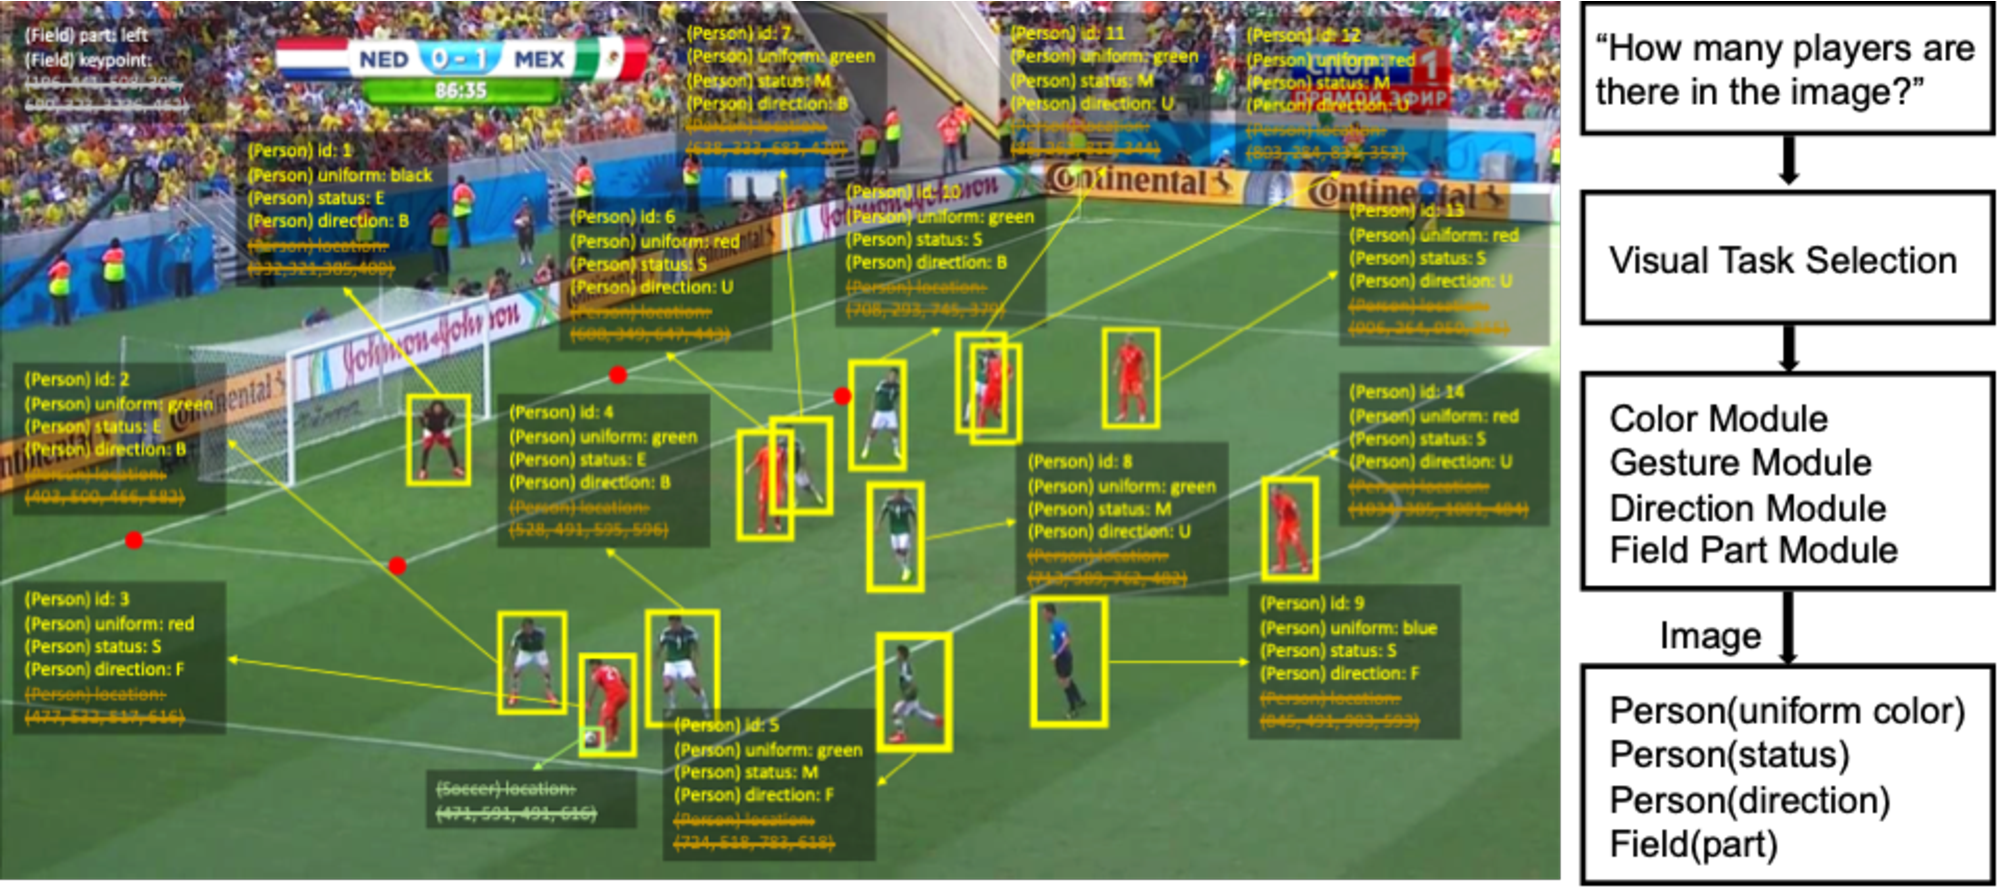
\includegraphics[width=\columnwidth]{figures/motivation.eps}
\caption{The image is about soccer match, where each person object is associated with attributes: id, uniform color, status (\underline{S}tanding, \underline{M}oving, \underline{E}xpansion), direction (\underline{B}acking, \underline{F}acing, \underline{N/A}), as well as location, and the soccer object is attributed with location. However, not all informations are necessary in answering one question, visual tasks are selected to achieve acquiring relevant information.%Part (b) shows a part of corresponding entity-attribute graph. Part (c) exhibits a $\nlq$ and its corresponding query graph $Q$. 
}
\vspace{-4ex}
\label{fig:example}
\end{figure}


\begin{example}
Figure~\ref{fig:example} depicts an image about a soccer match, where each object is associated with a set of attributes. A typical question may ask ``How many players are there in the image?''. Though simple, it is a challenging task to efficiently answer the query, since (1) traditionally, it often takes time to extract as much information as possible from the given image, and then answer the questions; while, only question related objects are needed; (2) information extracted from image alone is often insufficient to answer questions, hence missing values that are crucial for question answering should be inferred by certain reasoning techniques. \looseness=-1

To tackle the issues, one may (1) model input \ie image and question, with graph structures that can capture information from both image and question well, and ease question understanding and reasoning; (2) follow the work-flow given on the right hand side of Fig.~\ref{fig:example} to identify correct graph representation of the question, and a set of policies that are closely related to the question and used to guide forthcoming visual tasks; and (3) infer values \eg ``role'' of person objects (referee, goalkeeper or player) using well trained classification model.  
\end{example}

This example suggests that we address the \vqa problem by modeling inputs as graphs, leveraging techniques to guide question translation, visual processing, and do reasoning. While to do this, two critical questions have to be answered. (1) How to understand questions and carry out question related visual tasks? (2) How to infer crucial information to assist question answering?  


\vspace{2ex}
\stitle{Contributions.} In contrast to a majority of deep neural networks based \vqa techniques, which not only overlooks correlation between questions and images, but also lacks of necessary reasoning, we provide a novel approach that integrates question understanding and reasoning, for the \vqa problem. The main contributions of the paper are as follow.  

(1) We model images and questions as graphs, and propose to answer visual questions with graph matching. This new representation and answering scheme constitute the base of our techniques.  

(2) We introduce a method to guide question translation and visual processing based on reinforcement learning. That is, given a question, our method can identify its correct graph representation, and a set of policies to guide visual tasks in a more efficient manner. 

(3) We provide a method to infer missing values to answer questions. The reasoning task relies on a classifier, that is generated by offline training with supervised learning. 

4) We conduct extensive experimental studies to verify the performance of our method on both our curated \vqa dataset and a public \vqa dataset. We find that X, Y, and Z. 
\section{Related Work}
\label{sec-related-work}
\hspace{-2ex}
%Traditional approaches to the \vqa problem are mainly neural network based. In contrast, our approach consists of query understanding, query oriented object detection, and query answering. 
We categorize related work into following three parts. %: visual query answering, visual objects, and graph-based query answering. %\looseness=-1


\etitle{Visual query answering}. Current \vqa approaches are mainly based on deep neural works.  \cite{zhu2016visual7w} introduces a spatial attention mechanism similar to the model for image captioning. %In this method, a weight vector is computed and served as an additional input at each time step of the LSTM model. 
Instead of computing the attention vector iteratively, \cite{xu2016ask} obtains a global spatial attention weights vector which is then used to generate a new image embedding. 
\eat{
\cite{zhu2017structured} proposed to model the visual attention as a multivariate distribution over a grid-structured conditional random field on image regions, thus multiple regions can be selected at the same time. This attention mechanism is called structured multivariate attention in~\cite{zhu2017structured}.
}
There has been many other improvements to the standard deep learning method, \eg %compared to element-wise product or concatenation of the visual and textual representations,
\cite{fukui2016multimodal} utilized Multimodal Compact Bilinear (MCB) pooling to efficiently and expressively combine multimodal features. Another interesting idea is the implementation of Neural Module Networks~\cite{Andreas_2016,hu2017learning}, which decomposes queries into their linguistic substructures, and uses these structures to dynamically instantiate module networks. %Question-specific deep network is then assembled from these module networks that each solve one subtask. The layout of module networks can either be constructed from off-the-shelf parses~\cite{Andreas_2016}, or learned from the data~\cite{hu2017learning}.
\cite{teney2017graph} proposed to build graph over scene objects and question words. The visual graph is similar to ours, but the query graph differs. %\cite{teney2017graph} exploits the grammatical relations between words to generate query graph, while our method applies directed acyclic graph to represent query sentence. 
Note that the method \cite{teney2017graph} proposed is still a neural network based method as the structured representations are fed into a recurrent network to form the final embedding and the answer is again inferred by a classifier. %In contrast to recent works~\cite{Lu2015, Lu2016Hie}, we focus on single scene and involve reasoning. 


\etitle{Environment Exploration in Visual Field}. Reinforcement driven information acquisition is not only focusing on games~\cite{NIPS2017_7084,NIPS2002_2171,NIPS2017_7007} but also wildly applied in traditional vision domain.~\cite{DBLP:conf/cvpr/MathePS16} implement reinforcement learning in visual object detection, by presenting a novel sequential
models which accumulate evidence collected at a small set of
image locations to detect visual objects effectively.~\cite{DBLP:conf/cvpr/GoodrichA12} forms the facial detection problem into an adaptive learning process, by designing an approximate optimal control framework, based on reinforcement learning to actively search a visual field.~\cite{DBLP:conf/nips/MnihHGK14} proposed a novel recurrent neural network model which is capable to extract information from an image or video by adaptive selection for a sequence of regions or locations.~\cite{zhu2017icra} introduces reinforcement learning in the task of target-driven visual navigation. Other works aim at achieving {\color{red}XXX} based on algorithms~\cite{5596468,DBLP:conf/aaai/AbtahiF11}.

In visual and language domain, relevant work like~\cite{DBLP:conf/cvpr/RenWZLL17} achieves image captioning with Embedding Reward. Reinforcement learning preserves ability to effectively select preferred actions, which benefits the system in decomposing the problem into a few sub-tasks.


\eat{%20190305
{Visual Objects Processing}. Visual object detection as well as relationship identification are the preliminary tasks for not only \vqa but also image captioning~\cite{lu2016visual,yao2018exploring,teney2017graph}. %Many works in not in VQA but in image captioning has been done by firstly detect the visual objects~\cite{lu2016visual,yao2018exploring}, and then discover the relationship among them. 
Other works, \eg~\cite{yao2017boosting}, produce high-level attributes for input images, based on which further processing can be conducted. %These will help model to have a better understanding on properties of different regions/objects. 
These prior works show that detecting all visual objects, their attributes and relationships is very vital for resolving \vqa problem. %However, these work do not consider the relationship in detail, moreover it is quite hard to demonstrate spatial relationship (\eg close and far) and get relative distance between objects, due to perspective front view of the image.
%Even though, we  these techniques do not exactly solve the same problem as us, we get inspiration from them that, to explore the relationship between objects or image regions, we first need to detect all visual objects along with relevant attributes.
}%20190305


\etitle{Graph-based \vqa}. ~\cite{TuMLCZ14} proposes a framework to understand events and answer user queries, where underlying knowledge is represented by a spatial-temporal-causal And-Or graph (S/T/C-AOG). \cite{yi2018neural} recovers a structural scene symbolization from the image which is similar to graph representation, and learns a program trace from the question, which is later executed on the scene representation to obtain the answer. Our method differs in the way of answer retrieval by graph matching instead of program execution, furthermore, our method incorporates an inference graph to infer the missing values which turns out to improve the performance significantly. \cite{wang2018fvqa} conducts question-query mapping and then query-KB matching which is most similar to our method. Our model is different from \cite{wang2018fvqa} in that we implement reinforcement learning to make both visual processing and query generation more efficiently. Another strength of our method, again, is the introduction of inference graph which leads to powerful reasoning capability.

\eat{%20190318
Query answering has been extensively studied for graph data. In a nutshell, this work includes two aspects: query understanding, and query evaluation. We next review previous work on two aspects. 

\noindent (1) Queries expressed with natural languages are very user-friendly, but nontrivial to understand. Typically, they need to be structured before issuing over \eg search engine, knowledge graph, since structured queries are more expressive. There exist a host of works that based on query logs, human interaction and neural network, respectively. \cite{PoundHIW12} leverages query logs to train a classifier, based on which structured queries are generated.  \cite{ZhengC0YZ17} propose an approach to generate the structured queries through talking between the data (\ie the knowledge graph) and the user. \cite{YihCHG15} introduced how to generate a core inferential chain from a query with convolutional neural networks. As we only cope with a set of fixed queries, hence, we defer
the topic of query understanding to another paper, and focus primarily on the query evaluation. \looseness=-1

\noindent (2) To evaluate queries on graphs, a typical method is graph pattern matching. There has been a host of work
on graph pattern matching, \eg techniques for finding exact matches~\cite{cordella2004sub-full,subiso76}, inexact matches~\cite{ZouCO09,TianP08}, and evaluating \kw{SPARQL} queries on \kw{RDF} data~\cite{WagnerTLHS12}. Our work differs from the prior work in the following: (1) we integrate arithmetical and set operations in the query graph, and (2) we develop technique to infer missing values for query answering. \looseness=-1
}%20190318

% \subsection{Outline of the Paper}

% The rest of the paper is organized as follows. Section ~\ref{Preliminary} reviews notions and notations used in the paper. Section~\ref{sec-overview} outlines the framework our approach. Section \ref{sec-understanding} presents core components of our approach, \ie $\kw{VA}$ module (Section ~\ref{Visual Object}), inference module $\kw{IGC}$ (Section ~\ref{Inference}) and $\kw{GM}$ module (Section ~\ref{Query Answering}). Section ~\ref{Experiments} presents our experiments, followed by conclusion in Section ~\ref{Conclusion}.

\section{Overview of the Approach}
\label{sec-overview}

%%%%%%%%%%%%%%%
\begin{figure*}[tb!]
\vspace{-1ex}
\centerline{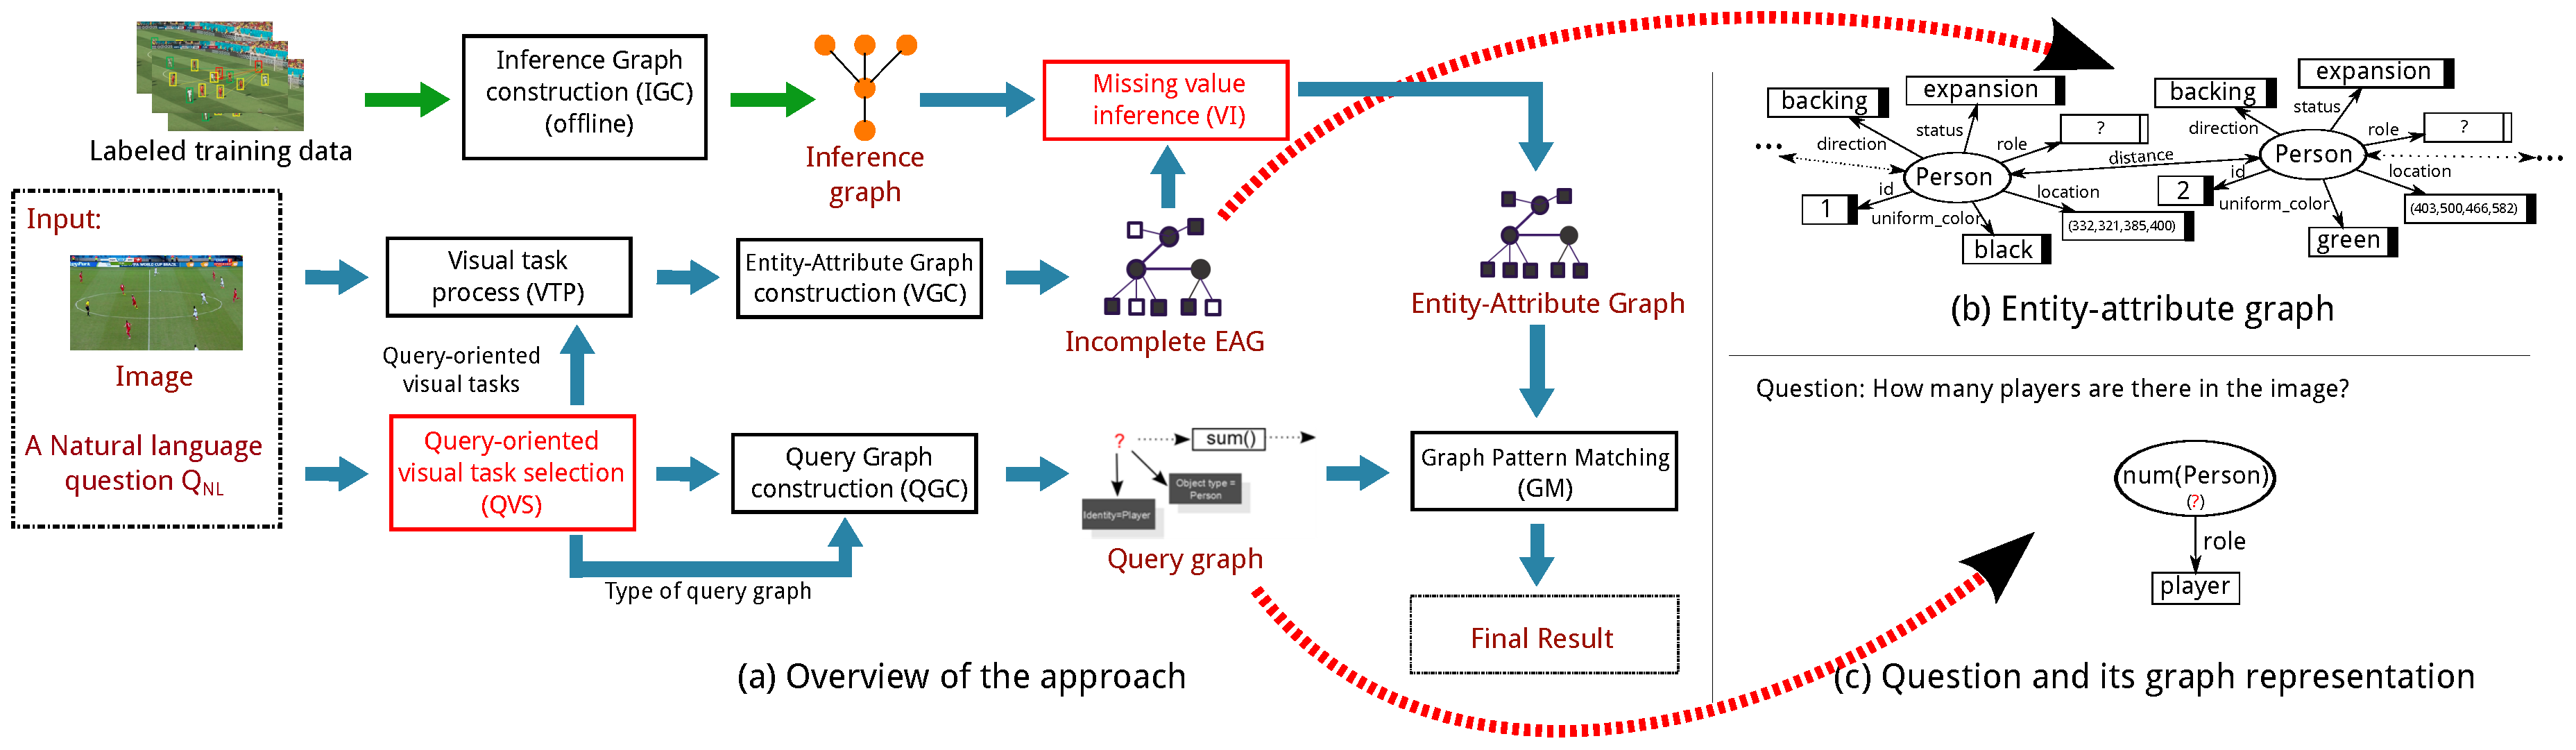
\includegraphics[scale=0.28]{overview.eps}}
\caption{Overview of our approach, and graph-based representation of images and questions} \label{fig-overview}
\vspace{-2ex}
\end{figure*}
%%%%%%%%%%%%%%%%

We start from representations of images and questions, followed by the overview of our approach.


\subsection{Representation of Images and Questions}
\label{sec-representation}

We use the same representations as~\cite{peixi2019}. To make the paper self-contained, we cite them as follows (rephrased). 

\stitle{Entity-Attribute Graphs.} Entities are typically defined as objects or concepts that exist in the real world. An entity often carries attributes, that describe features of the entity. \looseness=-1

Assume a set ${\cal E}$ of entities, a set ${\cal D}$ of values, a set ${\cal P}$ of predicates indicating attributes of entities and a set $\Theta$ of types. 
Each entity $e$ in ${\cal E}$ has a {\em unique ID} and a {\em type} in $\Theta$.

An {\em entity-attribute} graph, denoted as \kw{EAG}, is a set of triples $t = (s, p, o)$, where {\em subject} $s$ is an entity in ${\cal E}$, $p$ is a {\em predicate} in ${\cal P}$, and {\em object} $o$ is either an entity in ${\cal E}$ or a value $d$ in ${\cal D}$. It can be represented as a directed edge-labeled graph $\eag=(V, E)$, such that (a) $V$ is the set of nodes consisting of $s$ and $o$ for each triple $t = (s, p, o)$; and (b) there is an edge in $E$ from $s$ to $o$ labeled by $p$ for each triple $t = (s, p, o)$. \looseness=-1


\eat{%20190305
We consider two types of equality:

\noindent (a) {\em node identity} on ${\cal E}$: $e_1\Leftrightarrow e_2$ if entities $e_1$ and $e_2$ have the same ID, \ie they refer to the same entity; and 

\noindent (b) {\em value equality} on ${\cal D}$: $d_1 = d_2$ if they are the same value.

In $\eag$, $e_1$ and $e_2$ are represented as the same node if $e_1\Leftrightarrow e_2$; 
similarly for values $d_1$ and $d_2$ if $d_1=d_2$.
}%20190305


An image can be represented as an \kw{EAG} with detected objects along with their detected attributes, and relationships among objects. This can be achieved via a few visual tasks. While \kw{EAG} generated directly after image processing is often incomplete, \ie it may miss some crucial information to answer queries. We hence refer to {\em entity-attribute graphs} with incomplete information as {\em incomplete entity-attribute graphs}, and associate nodes with white rectangles, to indicate the missing value of an entity or attribute in \kw{EAG}. 
\eat{\Cref{fig:example}(b) is an {\em incomplete entity-attribute graph}, in which square nodes representing person roles are associated with white rectangle. 
}

\stitle{Query Graphs.}  A query graph $Q(u_o)$ is a set of triples
$(s_Q, p_Q, o_Q)$, where $s_Q$ is either a variable $z$ or a function $f(z)$ taking $z$ as parameter, $o_Q$ is one of a value $d$ or $z$ or $f(z)$, and $p_Q$ is a predicate in ${\cal P}$. Here function $f(z)$ is defined by users, and variable $z$ has one
of three forms: (a) {\em entity variable} $y$, to map to an entity, (b)
{\em value variable} $y*$, to map to a value, and (c) {\em wildcard} $\_y$, to
map to an entity. Here $s_Q$ can be either $y$ or $\_y$, while $o_Q$ can
be $y$, $y*$ or $\_y$. Entity variables and wildcard carry a {\em type},
denoting the type of entities they represent. 

A query graph can also be represented as a graph such
that two variables are represented as the same node if they
have the same name of $y$, $y*$ or $\_y$; similarly for functions $f(z)$ and values $d$.
We assume \kwlog that $Q(x)$ is connected, \ie there exists
an undirected path between $u_o$ and each node in $Q(u_o)$.
In particular, $u_o$ is a designated node in $Q(u_o)$, {\color{red}denoting the query focus and labeled by ``?''}. %denoting an entity. Introduce functions.  \looseness=-1

%Take \cref{fig-overview} (c) as example. It depicts a query graph that is generated from query ``{\em How many players are there in the image?}''. Note that the ``query focus'' $u_o$ carries a function \kw{num}() that calculates the total number of {\em person} entities with {\em role} ``player''. 


\subsection{Approach Overview}
\label{sec-architecture}

% %%%%%%%%%%%%%%%
% \begin{figure*}[tb!]
% \vspace{-1ex}
% \centerline{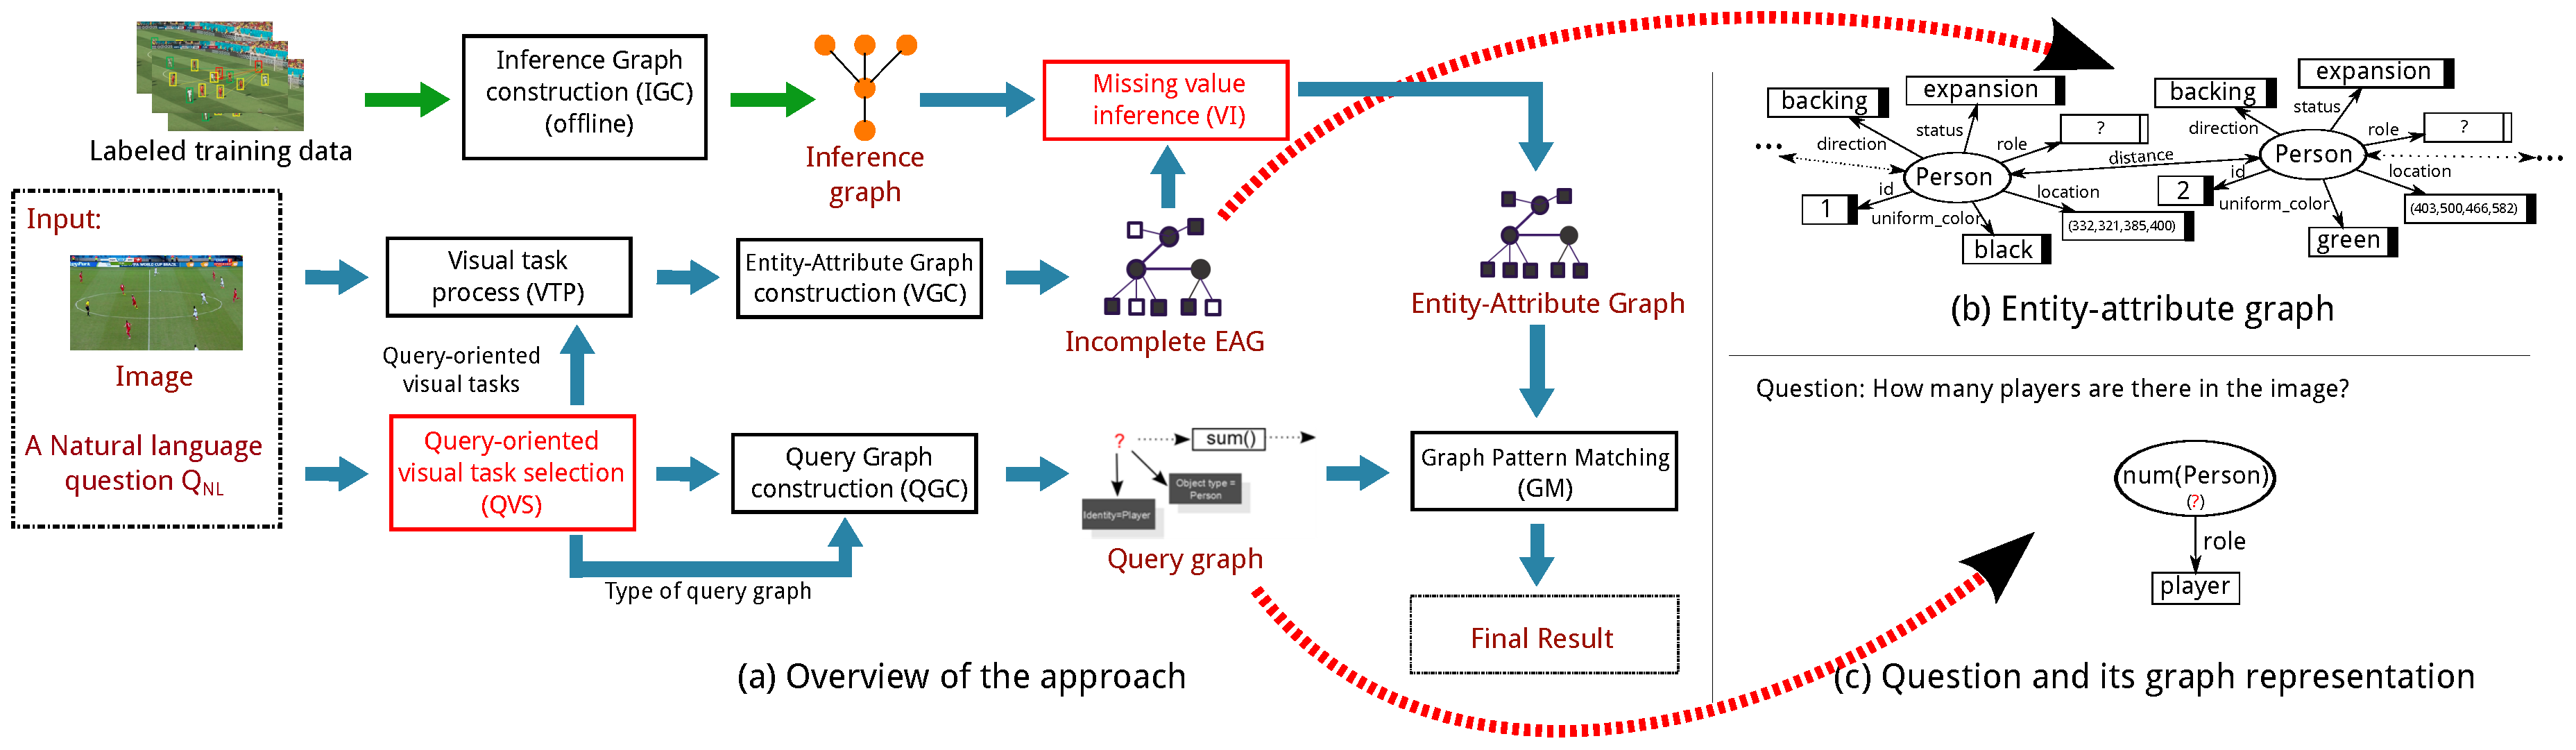
\includegraphics[scale=0.28]{overview.eps}}
% \caption{Overview of our approach, Entity Attribute Graph and Queries} \label{fig-overview}
% \vspace{-2ex}
% \end{figure*}
% %%%%%%%%%%%%%%%%


\eat{
Along the same lines as representations for images and questions, and graph pattern matching for question answering, raised in~\cite{peixi2019}, we propose a comprehensive approach as modeling of the \vqa problem. %answer a set of typical questions regarding soccer matches. 
}

\Cref{fig-overview} (a) presents the overview of our approach. In a nutshell, our approach takes an image and a natural language question $Q_{NL}$ as input, and answers questions with seven modules as following. (1) Upon receiving a question $Q_{NL}$, module \kw{QVS} identifies a set of visual tasks that are query-oriented and category of the query graph that corresponds to the input question, and passes tasks and category to modules \kw{VTP} and \kw{QGC}, respectively. (2) Guided by the list of tasks, module \kw{VTP} conducts visual tasks over the input image, and returns identified objects along with their attributes to module \kw{VGC}. (3) Module $\kw{VGC}$ constructs an entity-attribute graph $\eag$, using the identified objects and their attributes. Note that $\eag$ may be incomplete and hence unable to answer questions. (4) When $\eag$ is incomplete, module \kw{VI} infers missing value with a classifier $G_I$, denoted as {\em inference graph}, and produces an updated \kw{EAG} for question answering. (5) Module \kw{QGC} takes category of the query graph as input, and generates a query graph $Q(u_o)$. (6) After $Q(u_o)$ and $\eag$ are generated, module $\kw{GM}$ is invoked for matching computation, and returns final result. (7) In contrast to online computation that are processed by above modules, the module \kw{IGC} constructs {\em inference graphs} using labeled training data, offline. \looseness=-1

As some modules employ existing techniques, to emphasize our contribution, we will elaborate modules $\kw{QVS}$ and $\kw{VTP}$ in Section~\ref{sec-reinforcement-learning}, and modules \kw{VI} in Section~\ref{sec-reasoning}, with more details. \looseness=-1
\section{Question Oriented Visual Tasks}
\label{sec-reinforcement-learning}
In this section, we introduce how we do visual tasks that are in connection with questions. 




\subsection{Visual Processing}

In our approach, we build a structure which selects sub-tasks to form a policy which is based on queries. For instance, with the input \textit{which is the defending team?}, the system first predicts the corresponding visual action sequence, which are \textit{Human Module}, \textit{Gesture Module}, \textit{Direction Module}, \textit{Soccer Module}, \textit{Color Blob Module}, \textit{Field Part Module} and \textit{Graph Indicator}. Guided by such sequence, the image features are then extracted by operating relevant vision tasks. An overview is shown in Figure~\ref{fig:RLplot}.

\label{sec-visual-processing}
\begin{figure}[h]
\begin{center}
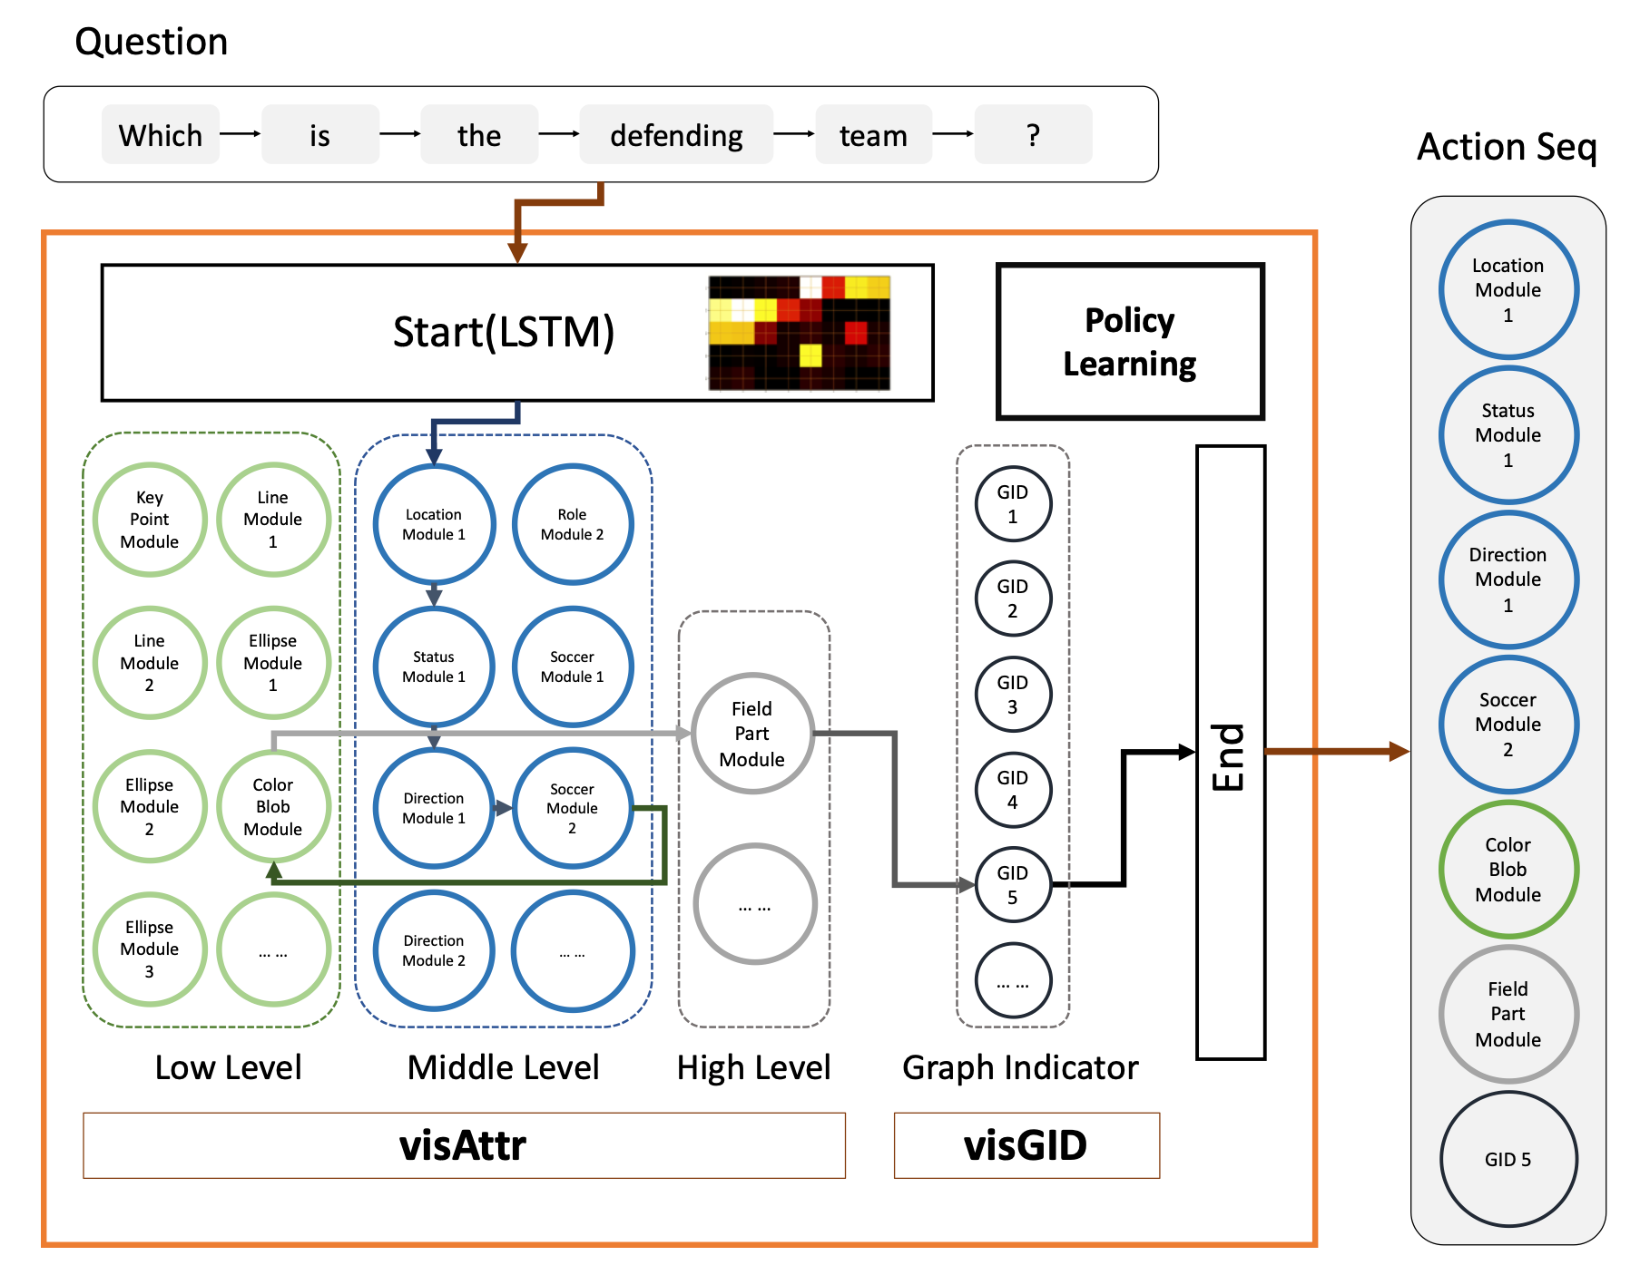
\includegraphics[width=\linewidth]{RLplot.pdf}
\end{center}
\caption{Visual Processing Strategy}
\label{fig:RLplot}
\end{figure}

\subsubsection{Multi-layer LSTM with Attention}
\label{sec-LSTM}
\hspace{\parindent}The task here is to predict the most suitable action modules sequence $\kw{a}$ by given questions $Q$ and preference $pre$. We form the problem of seeking effective answering strategy of question $Q$ and preference $pre$ as a sequence-to-sequence learning problem with attention mechanism. Inspired by~\cite{Bahdanau2016}, we input word feature of questions $w_i^q$, $i\in\|Q\|$ into a LSTM network which is regarded as an encoder and output $h_i$ as the hidden state for $i$th word in the question. By adding soft attention, the context vector $c_i$ is calculated by the following equations.


\begin{small}
\begin{equation} 
    c_i= \sum\nolimits_{j=1}^{\|Q\|} a_{ij}h_{ij}
\end{equation}
\begin{equation} 
    a_{ij}= \frac{exp(e_{ij})}{\sum\nolimits_{k=1}^{\|Q\|} exp(e_{ik})}
\end{equation}
\begin{equation} 
    e_{ij}= a(s_{j-1},h_i)
\end{equation}
\end{small}

\noindent where $h_i$ and $s_j$ are hidden states of encoder and decoder stage, respectively. Here $a_{ij}$ is the attention weights, with higher $a_{ij}$ in $(i, j)$ pair, the more attention will pay in this correlation, thus the $j$th output action $\kw{a}_i$ module will be more influenced by the $i$th input word $w_i^q$ in question. The decode part is similar as traditional recurrent neural networks (RNN). The following steps demonstrates decoding to get the joint distribution of action module sequence $\kw{A} = [\kw{a}_1,\dots,\kw{a}_t]$.

\begin{small}
\begin{equation} 
    p(\kw{A}|Q) = \Pi_{t\in\|\kw{A}\|}~p(\kw{a}_t|\{\kw{a}_1,\dots,\kw{a}_t\},c_i,Q)
\end{equation}
\begin{equation} 
    p(\kw{a}_t|\{\kw{a}_1,\dots,\kw{a}_t\},c_i,Q)= g(\kw{a}_{t-1},s_t,c_i,Q)
\end{equation}
\begin{equation} 
    s_t = f(s_{t-1},\kw{a}_{t-1},c_i)
\end{equation}
\end{small}
\noindent where $g(\cdot)$ is a nonlinear function which outputs the probability of action module \kw{a_{t}}. The probability distribution $p(\kw{A}|Q)$ is used to predict a maximum probability action module sequence by beam search during testing time.

Guided by this action sequence $[\kw{a}_1,\kw{a}_2,\kw{a}_3,\dots,\kw{a}_n]$, actions are selected from the following visual task pool, and comes into next session, visual task selection (\kw{VTS}).


\subsubsection{Visual Task Selection}
\label{sec-VTS}
\hspace{\parindent}\kw{VTS} is guided by the question feature, selecting target visual tasks from the visual task pool by Monte Carlo learning. The task pool is demonstrated in Table~\ref{table:visual_tasks}.


%\begin{table}[th]
%\centering 
%\scriptsize
%
%\begin{tabular}{|l|ll|l|}
%\hline
%visAttr & \multicolumn{1}{l|}{Level}  & Sub-task           & Descriptions                                                                                                                                 \\ \cline{2-4} 
%        & \multicolumn{1}{l|}{Low}    & Keypoint Module    & \multirow{3}{*}{\begin{tabular}[c]{@{}l@{}}To get detailed information of the \\ soccer field $F_{keypoint}$.\end{tabular}}                  \\ \cline{3-3}
%        & \multicolumn{1}{l|}{}       & Line Module        &                                                                                                                                              \\ \cline{3-3}
%        & \multicolumn{1}{l|}{}       & Ellipse Module     &                                                                                                                                              \\ \cline{3-4} 
%        & \multicolumn{1}{l|}{}       & Color Blob Module  & \begin{tabular}[c]{@{}l@{}}To detect blobs of different colors \\ among a region(whole soccer \\ field or a small bounding box).\end{tabular} \\ \cline{2-4} 
%        & \multicolumn{1}{l|}{Middle} & Location Module    & \begin{tabular}[c]{@{}l@{}}To detect the location of the \\ person $P_{location}$.\end{tabular}                                              \\ \cline{3-4} 
%        & \multicolumn{1}{l|}{}       & Status Module      & \begin{tabular}[c]{@{}l@{}}To get the person's gesture \\ $P_{status}$ (standing, moving, \\ expansion).\end{tabular}                        \\ \cline{3-4} 
%        & \multicolumn{1}{l|}{}       & Direction Module   & \begin{tabular}[c]{@{}l@{}}To get whether a person is facing \\ the goal or not $P_{direction}$.\end{tabular}                               \\ \cline{3-4} 
%        & \multicolumn{1}{l|}{}       & Uniform Module     & \begin{tabular}[c]{@{}l@{}}To get the uniform color of the \\ person $P_{uniform}$.\end{tabular}                                              \\ \cline{3-4} 
%        & \multicolumn{1}{l|}{}       & Soccer Module      & \begin{tabular}[c]{@{}l@{}}To detect the location of the \\ soccer $S_{location}$.\end{tabular}                                              \\ \cline{2-4} 
%        & \multicolumn{1}{l|}{High}   & Field Part Module  & \begin{tabular}[c]{@{}l@{}}To detect which part of the\\ soccer field is there in the \\ image $F_{part}$ .\end{tabular}                     \\ \hline
%visGID  &                             & Graph ID Indicator & \begin{tabular}[c]{@{}l@{}}To indicate which type of graph\\ will be used in the following \\process.
%\end{tabular}                          \\ \hline
%\end{tabular}
%\caption{\color{red}Visual Task Pool}
%\label{table:visual_tasks}
%\end{table}

%==========Table===================
\begin{table}[htbp]
	\centering 
	\scriptsize
%\begin{tabularx}{c| c| l | p{3cm} }
\begin{tabularx}{\linewidth}{ c | c| l | X }
	\Xhline{1pt}

%visAttr:
	\multirow{12}{*}[-5em]{visAttr} & {Level}  & Sub-task           & Descriptions                                                                                                                                 \\ \Xcline{2-4}{0.7pt}
	
	% first part
	& \multirow{4}{*}[-12pt]{Low} & Keypoint Module &  \multirow{3}{*}{ \parbox{3cm}{To get detailed information of the soccer field $F_\text{keypoint}$.} }  \\ \cline{3-3}
	& 					& Line Module   & \\\cline{3-3}
	& 					& Ellipse Module    & \\\cline{3-4}
	&					& Color Blob Module & {To detect blobs of different colors  among a region ( whole soccer field or a small bounding box).}\\ \cline{2-4}
	
	% second part
	& \multirow{5}{*}[-28pt]{Middle} & Location Module &  {To detect the location of the person $P_\text{location}$.}\\ \cline{3-4}
	&						  & Status Module   &   {To get the person's gesture  $P_\text{status}$ (standing, moving, expansion).} \\ \cline{3-4}
	&						  & Direction Module   &   {To get whether a person is facing the goal or not $P_\text{direction}$.} \\ \cline{3-4}
	&						  & Uniform Module    &   {To get the uniform color of the person $P_\text{uniform}$.} \\ \cline{3-4}
	&						  & Soccer Module  &  {To detect the location of the soccer $S_\text{location}$.}  \\ \cline{2-4}
	
	% third part
	& \multirow{1}{*}[-4pt]{High} & Field Part Module &  {To detect which part of the soccer field is there in the image $F_\text{part}$.} \\ \hline 
	
%visGID part
\multirow{1}{*}[-8pt]{visGID}  & \multicolumn{2}{c|}{\multirow{1}{*}[-8pt]{Graph ID Indicator}}	 &  {To indicate which type of graph  will be used in the following process.} \\
\Xhline{1pt}
\end{tabularx}
\caption{\color{red}Visual Task Pool}
\label{table:visual_tasks}
\end{table}
%==========Table===================

The pool is constructed by two parts, the first one is \textit{visAttr} which aims to discover the attribute of people, soccer, field and scene~\cite{peixi2019}, while the other one \textit{visGId} is an indicator showing the current question belongs to which graph type. There are three levels of \textit{visAttr}: low, middle and high, which represents different difficulty degree of the vision tasks. 

\begin{figure}[thb]
\centering
        \begin{subfigure}[b]{0.088\textwidth}
                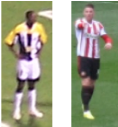
\includegraphics[width=\linewidth]{stand1.png}
                \caption{Standing}
                \label{fig:gull}
        \end{subfigure}\quad
        \begin{subfigure}[b]{0.127\textwidth}
                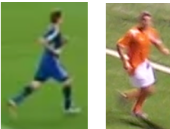
\includegraphics[width=\linewidth]{move1.png}
                \caption{Moving}
                \label{fig:gull2}
        \end{subfigure}\quad
        \begin{subfigure}[b]{0.166\textwidth}
                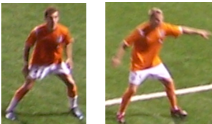
\includegraphics[width=\linewidth]{expand1.png}
                \caption{Expansion}
                \label{fig:tiger}
        \end{subfigure}
        \caption{Person status.}\label{fig:Person Status}
\end{figure}

For each vision task, the approach is not fixed, one task can be achieved by different methods with variance in time and accuracy. For instance, object detection based methods, like Faster R-CNN~\cite{Ren:2015:FRT:2969239.2969250}, R-FCN~\cite{DBLP:conf/nips/DaiLHS16}, SSD~\cite{DBLP:conf/eccv/LiuAESRFB16} or skeleton keypoints detection based method like~\cite{cao2017realtime} and~\cite{wei2016cpm} can be implemented as a set of status module methods, because all of them is able to localize and distinguish people who are moving, standing or with an expansion gesture (Figure~\ref{fig:Person Status}). Thus, the system is not only able to determine whether resembles a vision task module into action module sequence $[\kw{a}_1,\kw{a}_2,\kw{a}_3,\dots,\kw{a}_n]$, it can also select one specific approach under a vision task module, based on question and preference. For the preference, it is clarified in the next section.


\subsubsection{Time and Accuracy Term}
\label{sec-TimeAcc}
\hspace{\parindent} To better balance the accuracy and inference time for a given application, we proposed time and accuracy terms in loss function during training process.

\begin{small}
\begin{equation} 
    L_{\tau\alpha}(\theta) = \ell(\theta,\kw{A}|I, Q) + \gamma\sum_{i\in\|\kw{A}\|}\alpha(\kw{a_i}) + (1-\gamma)\sum_{i\in\|\kw{A}\|}\tau(\kw{a_i})
\end{equation}
\end{small}

\noindent where $\tau(\cdot)$ and $\alpha(\cdot)$represent the pre-tested inference time and inference accuracy, action module sequence \kw{A} samples from joint distribution $p(\kw{A}|Q)$, and here $\ell(\cdot)$ is the softmax loss over the predict score. For the preference term $\gamma$, it ranges from 0 to 1, which represents the preference over time and accuracy.

\subsubsection{Monte Carlo Methods}
\label{sec-MC}
\hspace{\parindent} The task now becomes a policy learning problem. Given a question and preference, output a policy containing a sequence of actions $[\kw{a}_1,\kw{a}_2,\kw{a}_3,\dots,\kw{a}_n]$. There is no ground truth for each steps, but only a final reward indicates that whether the prediction result is correct based on current policy. We involve the concept of Monte Carlo Methods to learn the policy which guides the vision tasks, and such policy network requires an extra reward value in loss.

\begin{small}
\begin{equation} 
    L_{policy}(\theta) = \sum\nolimits_{i\in\|A\|} log\pi(\kw{a}_{i}|Q,\theta)\ell(Q,\kw{A})
\end{equation}
\end{small}

\noindent where \kw{a_{i}} is the action will take, based on current status. $\pi(\cdot)$ is the policy function that maps status to actions, here, the policy is the probability of outputing next action module $\kw{a_{i}}$ based on current status. And $\ell(\cdot)$ here is the softmax loss based on the whole action module sequence $[\kw{a}_1,\kw{a}_2,\kw{a}_3,\dots,\kw{a}_n]$. Since all actions are discrete, which leads to non-differentiable, and back-propagation cannot be used. Policy gradient~\cite{Liu_2017_ICCV} is used here during training. The object function now becomes the combination of policy gradient loss $L_{policy}(\theta)$ with the time-accuracy-balanced loss $L_{\tau\alpha}$, and optimize it by backpropagation for $L_{\tau\alpha}$, while policy gradient for $L_{policy}(\theta)$.


\subsection{Construction of \kw{EAG}}
\label{sec-eag-construction}

After objects that are related to questions are identified, we construct a graph structure, denoted as \kw{EAG}, along the same line as~\cite{peixi2019}. 


\begin{example}
\label{exm-x1}
{\color{red} ADD AN EXAMPLE TO ILLUSTRATE PROGRESS IF NECESSARY!}
\end{example}

\section{Reasoning}
\label{sec-reasoning}

According to our observation,  an {\em incomplete} \kw{EAG} isn't well satisfying of answering the query because of the insufficient attributes.
To infer the hidden attributes, 
%In our proposed method, 
an inference graph is constructed accordingly.  
we briefly introduce the construction below. 

\subsection{Construction of Inference Graph}
To take advantage of the prior information and increase the generalization ability of the proposed model, our inference graph is constructed using Bayesian network.
Mathematically, Bayesian network \cite{friedman1997bayesian} can be described by a pair $\mathfrak{B}=<\mathcal{G},\varTheta_\mathcal{G}>$. 
Here, the notation $\mathcal{G}$ is a directed acyclic graph, of which the $i$-th vertex corresponds to a random variable $X_i$, and the edge between two connected vertexes indicates the dependency. 
Additionally, the second item $\varTheta_\mathcal{G}$ is a set of parameters used to quantify the dependencies in $\mathcal{G}$.
Denoted by $\text{Pa}(X_i)$ the attributes of the parents of $X_i$, 
the parameter of $X_i$ is represented by  $\theta_{X_i | \text{Pa}(X_i)} = P_\mathfrak{B}(X_i| \text{Pa}{(X_i)})$.
%We use the notation $\theta_{X_i | \text{Pa}(X_i)} = P_\mathfrak{B}(X_i| \text{Pa}{(X_i)})$ to denote the parameter of $X_i$, of which $\text{Pa}(X_i)$ is the attributes of the parents of $X_i$.
With the notations above, the joint probability distribution of Bayesian network is given by:

\begin{equation}\label{eq:BNOri}
P_\mathfrak{B}(X_1, \cdots, X_n) = 
\prod_{i=1}^{n} P_\mathfrak{B}(X_i| \text{Pa}{(X_i)})=
\prod_{i=1}^{n} \theta_{X_i | \text{Pa}(X_i)}
%\theta_{x_1|\text{Pa}_1(\mathbf{x})}\theta_{x_2|\text{Pa}_2(\mathbf{x})}\cdots \theta_{x_n|\text{Pa}_n(\mathbf{x})}
\end{equation}
\vspace{-1ex}

In our inference graph, the role of Bayesian network is to predict the object class when given the attributes $\{X_i\}_{i=1}^n$ as input. In the sense of probability, the object class is also a variable \cite{koller2009probabilistic}.
Defined by $X_0=Y$ the class variable, the network now has one extra vertex $X_0$.
In order to infer the class attribute, and according to the Bayesian rule, our problem becomes:

\vspace{-1ex}
\begin{align}\label{eq:BNWithCls}
\begin{split}
P_\mathfrak{B}(Y|{X}) & = 
\frac{ P_\mathfrak{B}(Y) P_\mathfrak{B}({X}|Y) }{P_\mathfrak{B}({X})}\\
&=\frac{ \theta_{Y|\text{Pa}({X}_0)} \prod_{i=1}^{n} \theta_{X_i|Y, \text{Pa}({X}_i)} }{ \sum_{y'\in \mathcal{Y}} \theta_{y'|\text{Pa}({X}_0)} \prod_{i=1}^{n} \theta_{X_i|y', \text{Pa}({X}_i)} }
\end{split}
\end{align}
where $\mathcal{Y}$ is the set of classes.

\begin{figure}[tb]
\centering
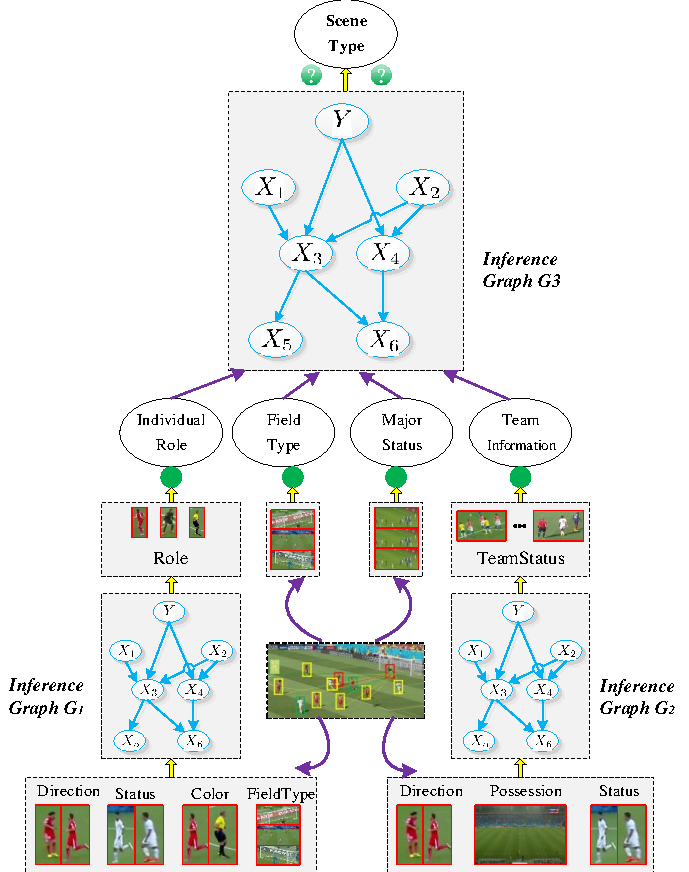
\includegraphics[width=\columnwidth]{inferGraph}
\caption{Schematic diagram of inference graph.}
\vspace{-4ex}
\label{fig:inferGraphWork}
\end{figure}

\subsection{Learning the Structure of Inference Graph}

In the context of Na\"{i}ve Bayes, 
the structure of $P_\mathfrak{B}(Y|{X})$ is simplified by taking the class variable as the root, and all attributes are conditionally independent when taking the class as a condition \cite{petitjean2018accurate}. As a consequence, the attribute class can be explicitly inferred by:

\begin{equation}\label{eq:BN-naiveBayes}
P_\mathfrak{B}(Y| {X}) = c \cdot \theta_Y \prod_{i=1}^{n}\theta_{X_i|Y}
\end{equation}
where $c$ is a scale factor that makes the calculation being a distribution: $c=\sum_{y'\in \mathcal{Y}}  \theta_{y'} \prod_{i=1}^{n}\theta_{X_i|y'}$.

Note from Eq.\eqref{eq:BN-naiveBayes} that Na\"{i}ve Bayes simplifies the complexity of Bayesian network. As can be validated by the experimental results, the simple model works excellently to our problem. 

Fig. \ref{fig:inferGraphWork} summarizes the processes of our inference graph, where three graphs are constructed according to the tasks involved. First, the role of a candidate is inferred, in which four different kinds of features are extracted from the scene image. Then, the team status is inferred through the second inference graph, but with different features as input. Next, we use the inferred information, along with the other information can be directly detected from the scene image, to infer the information of the whole scene.
The scene information is then fed into the incomplete \kw{EAG} so that a complete \kw{EAG} can be obtained. 

%\begin{figure}[tb!]
%\centering
%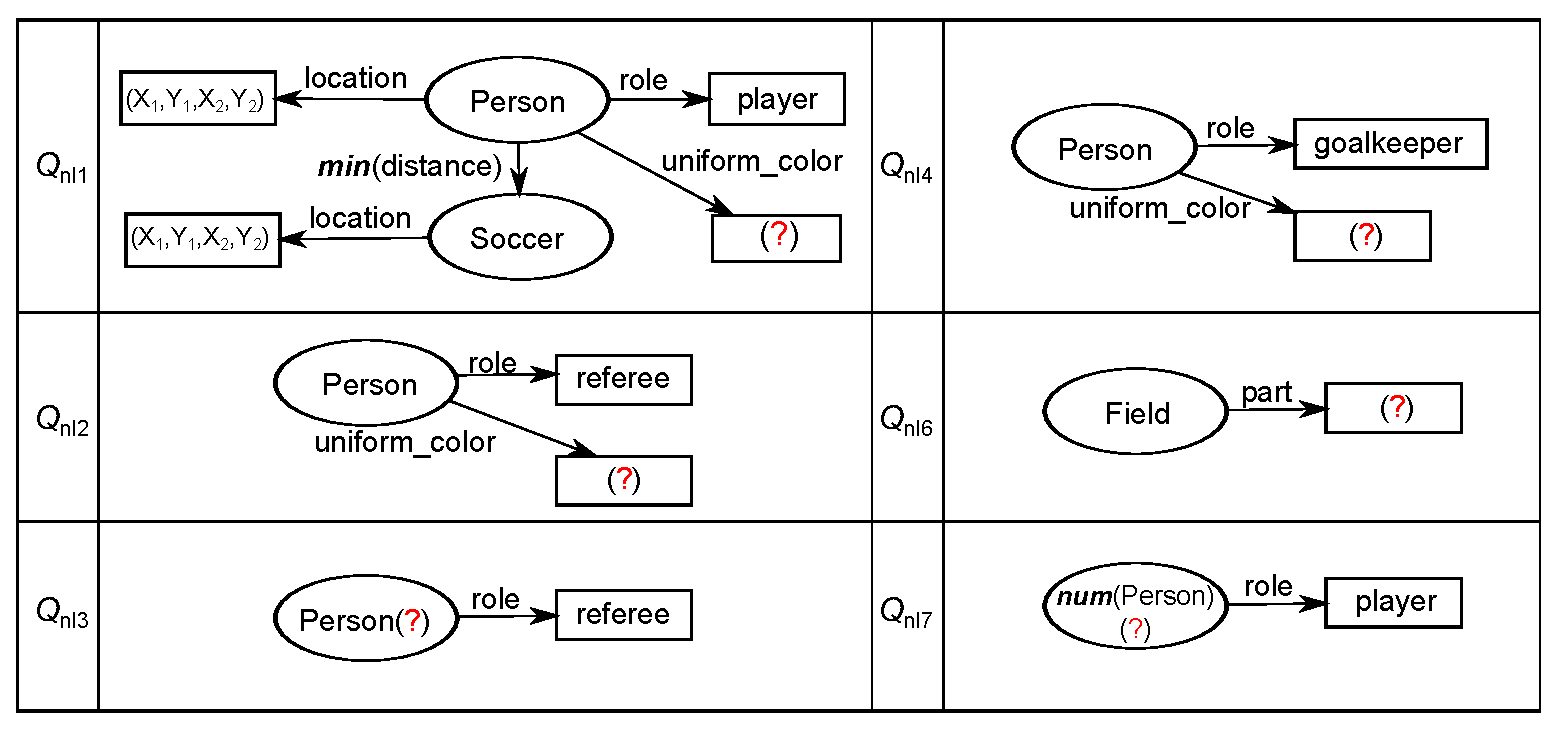
\includegraphics[width=\columnwidth]{queries.eps}
%\caption{Query graphs}
%\label{fig:queries}
%\end{figure}

\section{Experimental Studies}
\label{sec-expt}

In this section, we conduct four sets of experiments to evaluate (1) the generalization ability of our model, (2) the performance of our question oriented visual processing module (\kw{QVS} and \kw{VTP}), (3) the accuracy of our inference module (\kw{VI}), and (4) the overall performance of our model. \looseness =-1

\stitle{Experimental Setting}. %We report settings of experimental studies. 

\etitle{DataSet}. We used two data sets: (1) \kw{Soccer}~\cite{peixi2019} that we annotated; and (2) Visual-Genome~\cite{visualgenome}, one typical \vqa dataset. Over Visual-Genome dataset, we extracted 2852 images with subjects of baseball, tennis and soccer. 
For each dataset, we split it into two parts: Part$_I$, which accounts for 1/3 and used for testing, and Part$_{II}$ that accounts for 2/3 and used for training.   

\etitle{Questions}. We used two sets of questions: (1) the set of questions, listed in \cref{table:questions} for \kw{Soccer}; and (2) another set of questions for Visual-Genome. The questions for Visual-Genome are generated as following. We went over questions posed on Visual-Genome, extracted three kinds of typical questions, \ie ``what'', ``how many'' and ``where'' as base questions, and constructed in total 1179 questions with base questions, where 869 for ``what'' type, 259 for ``how many'' type, and 51 for ``where'' type. 

%==========Table===================
\begin{table}[thb]
	\renewcommand{\arraystretch}{1}
	\begin{center}
		\footnotesize		
		\begin{tabular}{c|c|c}
			\Xhline{1pt}
			Id & Question                                           & Difficulty \\ \Xhline{0.7pt}
			%$Q_{nl_1}$  & Who is this image about?                         & Hard       \\ \hline
			$Q_{nl_1}$  & Who is holding the soccer?                         & Easy       \\ \hline
			$Q_{nl_2}$  & What is the uniform color of the referee?           & Easy       \\ \hline
			$Q_{nl_3}$  & Is there any referee in the image?                 & Easy       \\ \hline
			$Q_{nl_4}$  & Which team does the goalkeeper belong to?          & Medium       \\ \hline
			$Q_{nl_5}$  & Who is the defending team?                         & Medium       \\ \hline
			$Q_{nl_6}$  & Which part of the field are the players being now? & Hard       \\ \hline
			$Q_{nl_7}$  & How many players are there in the image?           & Hard     \\ \hline
			$Q_{nl_8}$  & Is this image about corner kick?                   & 
			\\ \hline
			$Q_{nl_9}$  & Is this image about free kick?                     & 
			\\ \hline
			$Q_{nl_{10}}$  & Is this image about kick off?                  & 
			\\ \hline
			$Q_{nl_{11}}$  &  Is this image about penalty kick?             &
			\\ \hline
			\eat{
			\multirow{2}{*}{$Q_{nl_8}$ }
			& Is this image about corner kick?           &  \multirow{2}{*}{\color{red}??}  \\ 
			& {\color{red}(If not, just list the correct one.)}  & \\ \hline
			
			\multirow{2}{*}{$Q_{nl_{9}}$}  &  Is this image about free kick?  &  \multirow{2}{*}{\color{red}??}    \\ 
			& {\color{red}(If not, just list the correct one.)}  &  \\ \hline
			
			\multirow{2}{*}{$Q_{nl_{10}}$}  &  Is this image about kick off?  &  \multirow{2}{*}{\color{red}??}    \\ 
			& {\color{red}(If not, just list the correct one.)}  &  \\ \hline
			
			\multirow{2}{*}{$Q_{nl_{11}}$}  &   Is this image about penalty kick?  &  \multirow{2}{*}{\color{red}??}    \\ 
			& {\color{red}(If not, just list the correct one.)}  &  \\ %\hline
			\Xhline{1pt}
			}
		\end{tabular}
		\caption{A set of questions}
		\label{table:questions}
	\end{center}
\end{table}
%==========Table===================


\subsection{Generalization Ability of the Model}

To show the generalization ability of our model, we compared accuracy of our model with state-of-the-art methods CNN+LSTM~\cite{VQA}, HieCoAttenVQA~\cite{Lu2016Hie} and Learning2Reason~\cite{hu2017learning}, via changes of training data. For comparison purpose, we enrich training data with those questions taking the same semantic meaning. For example, besides $Q_{nl5}$, we add following questions: \textit{Who is attacking team?}, \textit{"What is the uniform color of the defending team?"} and \textit{"What is the uniform color of the attacking team?"}, that have the same semantic meaning as $Q_{nl5}$ in training data. As shown in \cref{table:genralization}, our model always outperforms others, and moreover, is influenced least by varied training data, than other methods. The reason is that all the visual task selection is question oriented, which leads to unfixed network structure, also, the graph-based method preserves better reasoning capability, comparing with memorizing statistic correlations between images and answers.


\eat{
To test the generalization of our method, we enlarge the training set by more various question with same meaning. For instance, the original question of $Q_{nl5}$ is \textit{"Who is the defending team?"}, we add three more similar question asking \textit{Who is attacking team?}, \textit{"What is the uniform color of the defending team?"} and \textit{"What is the uniform color of the attacking team?"}. Unlike state-of-the-art methods answering questions in~\cite{peixi2019}, adding generalization and variation in question would not dramatically change the performance, it is because the structure is not fixed, all the visual task selection is query oriented. For~\cite{hu2017learning}, even though the network is not fixed, the answering part is based on neural network, and essentially it also learns the statically correlation, which leads to the weakness in logical reasoning. The result is is shown in \cref{table:genralization}.
}

\begin{table}[h]
	\small
	\begin{tabular}{|l|l||l|l|}
		\hline
		\multicolumn{2}{|l||}{Various Training Questions} & \multicolumn{2}{l|}{Original Training Questions} \\ \hline \hline
		Methods                  & Acc(\%)            & Methods                   & Acc(\%)             \\ \hline
		CNN+LSTM                    & 28.14              & CNN+LSTM                     & 46.40               \\ \hline
		HieCoAttenVQA               & 31.92              & HieCoAttenVQA                & 49.11               \\ \hline
		Learning2Reason             & 38.00              & Learning2Reason              & 51.08               \\ \hline
		Ours                        & 64.02              & Ours                         & 66.75               \\ \hline
	\end{tabular}
	\caption{Generalization ability of our model} \label{table:genralization}
\end{table}


\subsection{Performance of Visual Processing}

Efficiency is one crucial factor to evaluate the performance of a \vqa model. 
In light of this, we evaluate the running time over accuracy by using state-of-the-art methods CNN+LSTM~\cite{VQA} HieCoAttenVQA~\cite{Lu2016Hie}, Learning2Reason~\cite{hu2017learning} and AllTasks~\cite{peixi2019}. To measure the efficiency of \vqa models, we use ``CPU Time'' to represent the total running time of entire progress of question answering. 

The results shown in \cref{fig:TimevsAcc} tell us that: (1) state-of-the-art methods perform efficiently, with running time less than 300 milliseconds, while their accuracy are all below 40\%, showing that the methods are not applicable in practice; (2) AllTasks always has the highest and steady accuracy, \eg 65.86\%, since it processes all the visual related tasks without selection, paying the price of unexpected and long running time; and (3) our module finds a balance between efficiency and accuracy. For example, with $\gamma=0.99$, our reinforcement learning based module spends, on average, 680 ms to answer questions, with accuracy 64.02\%, which is 35.88\%, 32.10\% and 26.02\% higher than that of CNN+LSTM, HieCoAttenVQA, and Learning2Reason, respectively. Moreover, when running time decreases, the accuracy decreases either, which is as expected.

\begin{figure}[h]
	\begin{center}
		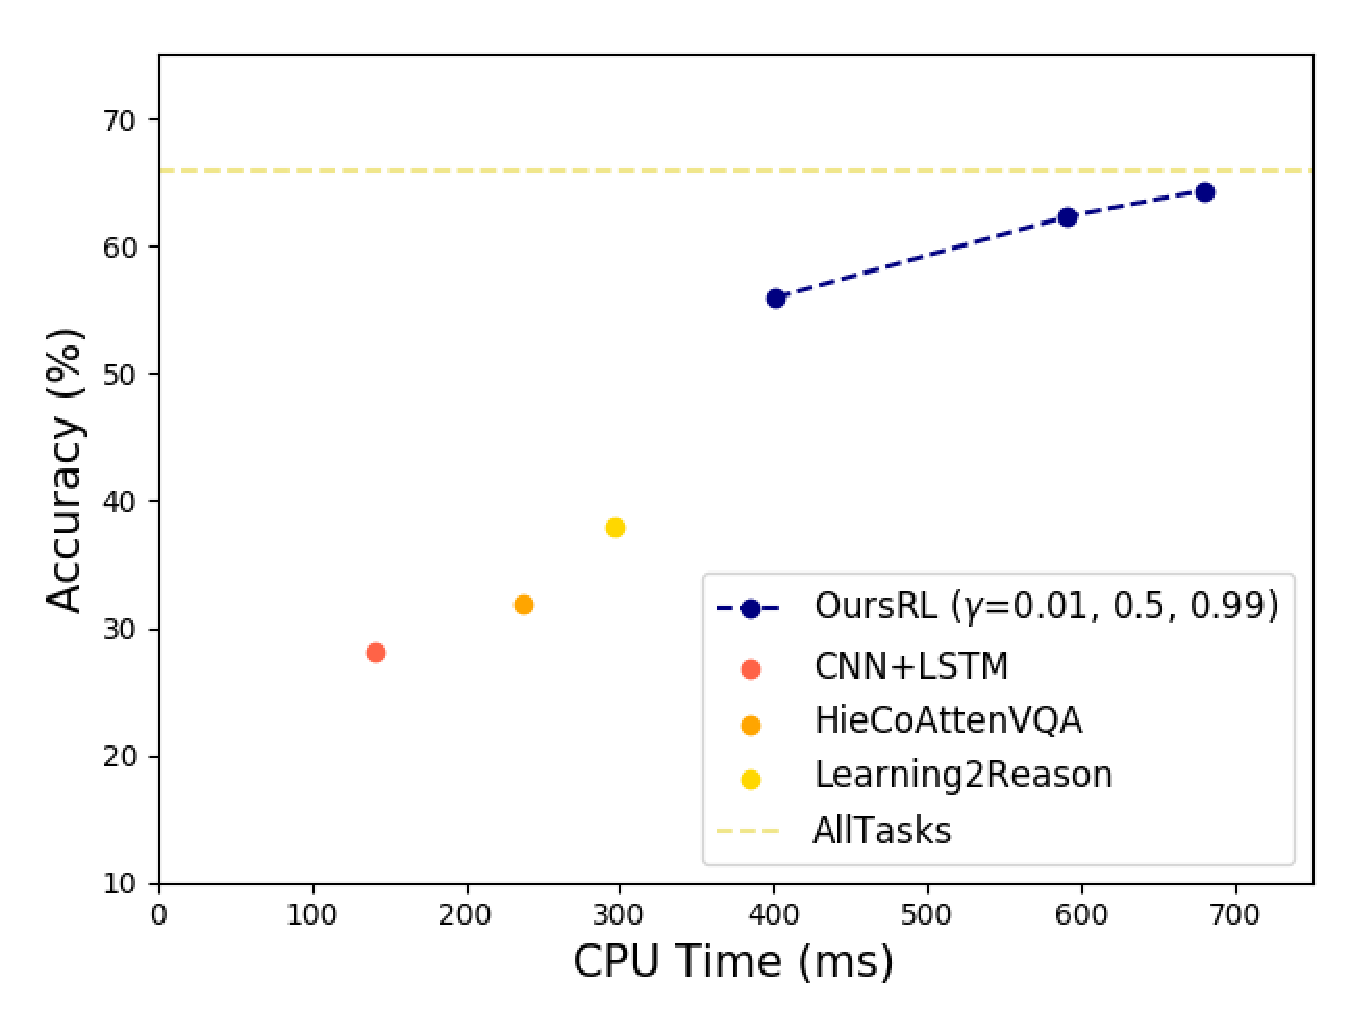
\includegraphics[width=0.75\linewidth]{figures/TimevsAcc.eps}
	\end{center}
	\vspace{-3ex}
	\caption{Balance between running time and accuracy}
	\vspace{-2ex}
	\label{fig:TimevsAcc}
\end{figure}


\eat{
	\cref{tab:AccuracyCmp} lists the time cost and accuracy results among different approaches. For CNN+LSTM, HieCoAttenVQA, and Learning2Reason, their systems work quite efficient with responding time less than 300ms. But the accuracies of these three approaches are lower than 40\%, which is unacceptable. Whereas, the system similar to \cite{peixi2019} outperforms all other methods and reaches 65.86\% accuracy, but it costs much more time. Our approach is able to keep balance between effectiveness and efficiency. For effectiveness, our approach achieves 64.02\% accuracy, which is 35.88\%, 32.10\% and 26.02\% higher than results of CNN+LSTM, HieCoAttenVQA, and Learning2Reason, respectively. For efficiency, our approach can reduce the inference time by choosing a small value of $\gamma$.
	
	
	We compare our approach to the state-of-the-art systems, \ie CNN+LSTM~\cite{VQA} HieCoAttenVQA~\cite{Lu2016Hie}, and Learning2Reason~\cite{hu2017learning}. 
	
	%==========Table===================
	\begin{table}[htbp]
		\renewcommand{\arraystretch}{1}
		\begin{center}
			\small		
			\begin{tabular}{c|*{2}{c}}
				\Xhline{1pt}
				& Time (ms)  & Accuracy (\%) \\ \Xhline{0.7pt}
				CNN+LSTM  &  141  &  28.14\\
				HieCoAttenVQA  &  237  &  31.92\\
				Learning2Reason  &  297  &  38.00\\
				Ours (Without RL)  &  N/A  &  65.85\\
				Ours ($\gamma=0.01$)  &  401  &  55.92\\
				Ours ($\gamma=0.50$)  &  591  &  62.29\\
				Ours ($\gamma=0.99$)  &  680  &  64.02\\
				\Xhline{1pt}
			\end{tabular}
			\caption{Inference time and accuracy comparison.}
			\label{tab:AccuracyCmp}
		\end{center}
	\end{table}
	%==========Table===================
}


\subsection{Performance of Inference} 
\eat{
	\begin{figure}[tb!]
		\centering
		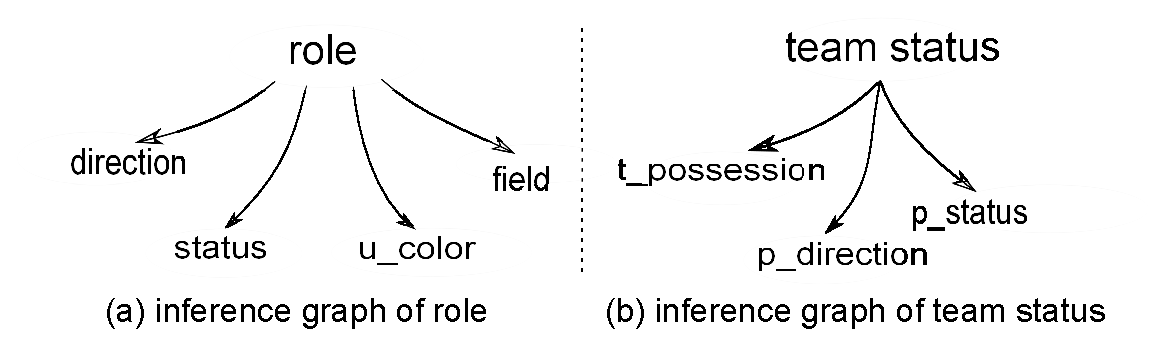
\includegraphics[width=\columnwidth]{PredictNB.eps}
		\vspace{-2ex}
		\caption{Inference graphs}
		\vspace{-2ex}
		\label{fig:inferGraph}
	\end{figure}
}

Accuracy is another crucial performance criteria of \vqa systems. In contrast to end-to-end systems, the accuracy of our model is partly influenced by the inference quality. Hence, it is of great importance to see how accuracy is influenced by our inference module (\kw{VI}). Prior work~\cite{peixi2019} already showed performance of their inference module \wrt a set of fixed questions on Soccer dataset. Here, we learn an inference graph for questions $Q_{nl8},Q_{nl9},Q_{nl10}$ and $Q_{nl11}$ regarding field scene from Soccer dataset, and a set of inference graphs for answering questions on Visual-Genome dataset. \looseness=-1

To evaluate accuracy, we follow F-measure~\cite{Fmeasure}, and define our accuracy metric as following:


\noindent $\kw{Acc}=2\cdot (\kw{recall}\cdot \kw{precision})~/~(\kw{recall}+\kw{precision})$;

\noindent $\kw{recall}=\#\kw{true}\_\kw{value}\_\kw{inferred}~/~\#\kw{true}\_\kw{value}\_\kw{instance}$;

\noindent $\kw{precision}=\#\kw{true}\_\kw{value}\_\kw{inferred}~/~\#\kw{inferred}\_\kw{instance}$.


Here $\#\kw{true}\_\kw{value}\_\kw{inferred}$ is the number of all the instances, whose attribute $A$ is inferred correctly as $``v"$,  $\#\kw{true}\_\kw{value}\_\kw{instance}$ is the number of all the instances with attribute $A$ of value $``v"$, and $\#\kw{inferred}\_\kw{instance}$ indicates the total number of instances whose attribute $A$ is inferred as $``v"$. \looseness=-1




\eat{
\stitle{Accuracy of Role}. 

Based on questions and image characteristics, four variables including $direction$, $status$, $field$, and $unique\_color$ (abbr. $u\_color$) are adopted to calculate conditional probabilities. The inference graph is shown in \cref{fig:inferGraph}. Note that the domain of variables $direction$, $status$ and $field$ are given in {\color{red}Table ????}, while variable $u\_color$ can have one of two values, to indicate whether a person object has the unique uniform color (=``$U$'') or not (=``$M$'').

%==========Table===================
\begin{table}[htbp]
	\renewcommand{\arraystretch}{1}
	\begin{center}
		\small		
		\begin{tabular}{c|*{3}{r}}
			\Xhline{1pt}
			Role & Precision  & Recall  & Acc \\ \Xhline{0.7pt}
			Goalkeeper  &  94.4  &  85.5  &  89.8\\
			Referee  &  87.4  &  82.8  &  85.0\\
			Player  &  98.8  &  99.3  &  99.0\\
			\Xhline{1pt}
		\end{tabular}
	\caption{Inference accuracy of role (\%).}
	\label{tab:InferAccRole}
	\end{center}
\end{table}
%==========Table===================

Using the conditional probabilities, $VI$ {\color{red}(???)} infers role of each person object. The inference accuracy is shown in \Cref{tab:InferAccRole}. It is easy to find that the inference accuracy for role player reaches 99\%, which is highest among all roles. And the accuracy for different roles are all above 85\%.

\stitle{Accuracy of Team Status}

%===================== figure ============
\begin{figure}[!bth]
	%\scriptsize
	\centering	
	\begin{minipage}[b]{\linewidth}
		\centerline{\includegraphics[width=0.5\linewidth]{example-image-a}}
	\end{minipage}\hfill
	\caption{Attributes of team inference graph.}
	\label{fig:AtribTeamGraph}
\end{figure}
%===================== figure ============

%==========Table===================
\begin{table}[htbp]
	\renewcommand{\arraystretch}{1}
	\begin{center}
		\small		
		\begin{tabular}{c|*{3}{r}}
			\Xhline{1pt}
			 Team Status & Precision  & Recall  & Acc \\ \Xhline{0.7pt}
			Defending  & 89.8 &	74.2 &	81.3\\
			Attacking  &  79.1 & 	92.1 &	85.1\\
			\Xhline{1pt}
		\end{tabular}
		\caption{Inference accuracy of team status (\%).}
		\label{tab:InferAccTeam}
	\end{center}
\end{table}
%==========Table===================

\Cref{tab:InferAccTeam} gives the performance of our approach for inferring team status. The accuracy of defending and attacking are above 80\%. To be specific, the accuracy for inferring if a team is attacking achieves 85.1\%, which is higher than the inference accuracy for defending status detection by 3.8\%.
}


%===================== figure ============
\begin{figure}[!bth]
	%\scriptsize
	\centering	
	\begin{minipage}[b]{\linewidth}
		\centerline{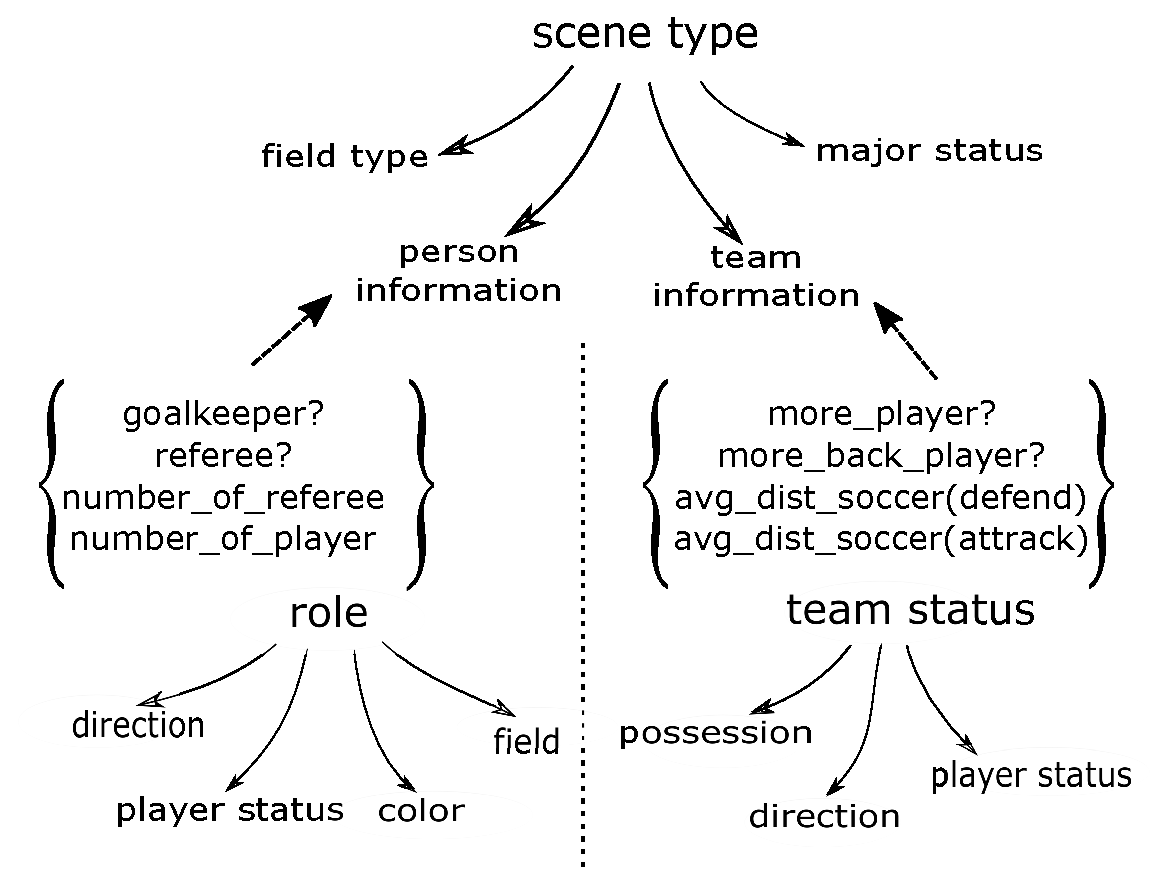
\includegraphics[width=1\linewidth]{attribtes_infGraph}}
	\end{minipage}\hfill
	\caption{Attributes of scene inference graph.}
	\label{fig:AtribSceneGraph}
\end{figure}
%===================== figure ============


\stitle{Accuracy of Field Scene}. We choose four typical field scenes, \ie corner kick, free kick, penalty kick and kick-off, as  which have distinct scene features. Practically, (1) corner kick scene always shows that a single player kicks the ball within a one-yard radius of the corner flag and most of players gather at the penalty field. (2) Free kick happens with a defensive wall mostly. (3) It is much typical for the penalty kick scene because most of players are out of penalty area except the penalty kicker and goalkeeper with football in the penalty spot. (4) For kick-off scene, the soccer appears in the center spot and is surrounded by players from two opposing teams. Based on these observations, we design an inference graph which is shown in \cref{fig:AtribSceneGraph}.

Using inference graph shown in \cref{fig:AtribSceneGraph}, we have results
showing accuracy of inference. 
%Inference results are indicated in \Cref{tab:InferAccField} based on inference graph in \cref{fig:AtribSceneGraph}. 
As can be seen, the inference accuracy of corner kick, free kick, kick-off and penalty kick are 59.57\%, 63.16\%, 85.94\% and 60.00\%, respectively, among which the scene of kick off gains the highest inference accuracy.
 

%==========Table===================
\begin{table}[htbp]
	\renewcommand{\arraystretch}{1}
	\begin{center}
		\small		
		\begin{tabular}{c|*{3}{r}}
			\Xhline{1pt}
			Scene Type & Precision  & Recall  & Acc \\ \Xhline{0.7pt}
			Corner-kick &  59.57  &  68.29  &  63.64\\
			Free-kick  &  63.16  &  58.54  &  60.76\\
			Kick-off &  85.94  &  82.09  &  83.97\\
			Penalty-kick  &  60.00  &  60.00  &  60.00\\
			\Xhline{0.7pt}
			Avg.  &  71.28  &  70.73  &  70.89\\
			\Xhline{1pt}
		\end{tabular}
	\caption{Inference accuracy of four typical scenes (\%).
		% Here ``Co'', ``Fr'', ``Ki'' and ``Pe'' indicate corner kick, free kick, penalty kick and kick-off, respectively.
	}
	\label{tab:InferAccField}
	\end{center}
	\vspace{-3ex}
\end{table}
%==========Table===================


In addition, we compare our approach with NuSVC, MLP, and AdaBoost in \cref{tab:AccFieldCmp}. The results show that the average accuracy of our approach is higher than that of NuSVC and AdaBoost by 4.49\% and 5.97\% respectively, and slightly better than that of MLP.

%==========Table===================
\begin{table}[htbp]
	\renewcommand{\arraystretch}{1}
	\begin{center}
		\small		
		\begin{tabular}{c|*{3}{r}}
			\Xhline{1pt}
			 & Precision  & Recall  & Acc \\ \Xhline{0.7pt}
			NuSVC  &  68.30  &  65.85  &  66.40\\
			MLP  &  70.80  &  \textbf{70.73}  &  70.32\\
			AdaBoost  &  65.50  &  65.24  &  64.92\\ %\Xhline{0.7pt}
			Ours  &  \textbf{71.28}  &  \textbf{70.73}  &  \textbf{70.89}\\
			\Xhline{1pt}
		\end{tabular}
	\caption{Accuracy comparison of field scene (\%)}
	\label{tab:AccFieldCmp}
	\end{center}
	\vspace{-3ex}
\end{table}
%==========Table===================



%\stitle{Accuracy of Kick-Off}. {\color{red} SHOW INFERENCE GRAPH AND RESULT TABLE!}
%
%\stitle{Accuracy of Penalty Kick}. {\color{red} SHOW INFERENCE GRAPH AND RESULT TABLE!}
%
%\stitle{Accuracy of Corner Kick}. {\color{red} SHOW INFERENCE GRAPH AND RESULT TABLE!}
%
%\stitle{Accuracy of Attacking Free Kick}. {\color{red} SHOW INFERENCE GRAPH AND RESULT TABLE!}
%
%\stitle{Accuracy of Balls}. {\color{red} Over new dataset. SHOW INFERENCE GRAPH AND RESULT TABLE!}

\subsection{Overall Performance}
\label{sec-overall-performance}
%We use the same question setting as~\cite{peixi2019}, compared the following state-of-the-art methods: \cite{VQA},and~\cite{hu2017learning} with our method ($\gamma$=0.99), the overall performance is shown in Table~\ref{table:stateofart}. 

We compare our approach with the following state-of-the-art methods: CNN+LSTM, HieCoAttenVQA, and Learn2Reason, using Soccer and Visual-Genome dataset. 
\Cref{table:stateofartSoc} lists results on Soccer. We find that (1) the average accuracy of our approach is higher than that of CNN+LSTM, HieCoAttenVQA and Learn2Reason by 20.35\%, 17.64\% and 15.67\%,  respectively; (2) our approach is typically effective in answering hard problems, \eg with improvement over 60\% for $Q_{nl6}$. 
Consider that questions $Q_{nl8}-Q_{nl11}$ are all about field scene, while more than 90\% images of Soccer dataset are categorized as normal scene. For the fair comparison, we extract images that are categorized as one of four field scenes, and apply our approach over this subset of dataset. As shown in \cref{table:stateofartSoc}, our approach substantially outperforms others, which further verifies the advantage our approach preserves. 
Results on Visual-Genome are given in \cref{table:stateofartVisGen}, from which we find: (1) for ``what'' and ``where'' questions, Learn2Reason performs best, while performances of four methods are quite close; (2) for ``how many'' questions, our method performs much better than others; and (3) the average accuracy our method  surpasses CNN+LSTM, HieCoAttenVQA and Learn2Reason by 12.93\%, 11.74\% and 9.7\%, respectively, which further verifies its advantage. 
\eat{
To evaluate the generalization of the proposed scheme, we measure its accuracy on Visual Genome Dataset. Results in \cref{table:stateofartVisGen} show that our approach can handle different types of questions, and the overall performance of our approach surpasses CNN+LSTM, HieCoAttenVQA and Learn2Reason by 12.93\%, 11.74\% and 9.7\%, respectively.
}
\eat{
The results are listed in \cref{table:stateofartSoc}. The average accuracy using our approach is higher than that of CNN+LSTM, HieCoAttenVQA and Learn2Reason by 20.35\%, 17.64\% and 15.67\%,  respectively. 
}

%==========Table===================
\begin{table}[htbp]
	\renewcommand{\arraystretch}{1}
	\begin{center}
		\small		
		\begin{tabular}{c|*{4}{c}}
			\Xhline{1pt}
			& CNN+LSTM & HieCoAtten & Learn2Reason & Ours \\ \Xhline{0.7pt}
			$Q_{nl1}$ & 44.23    & 43.62         & 31.12        & \textbf{64.86} \\ 
			$Q_{nl2}$ & 71.31    & \textbf{77.66}         & 9.4          & 63.74 \\ 
			$Q_{nl3}$ & 74.58    & \textbf{83.78}         & 83.21        & 70.00 \\ 
			$Q_{nl4}$ & 40.48    & 39.29         & 51.92        & \textbf{62.14} \\ 
			$Q_{nl5}$ & 49.19    & 49.90         & 30.78        & \textbf{62.58} \\ 
			$Q_{nl6}$ & 20.56    & 18.70         & 30.0         & \textbf{93.33} \\ 
			$Q_{nl7}$ & 11.08    & 12.63         & 36.69        & \textbf{50.60} \\\Xhline{0.7pt} 
			$Q_{nl8}$ &     &           &          &   \\
			$Q_{nl9}$ &     &           &          &   \\
			$Q_{nl10}$ &      &           &          &   \\
			$Q_{nl11}$ &      &           &          &   \\ \Xhline{0.7pt} 
			Avg.       & 46.40    & 49.11         & 51.08        & \textbf{66.75} \\
			\Xhline{1pt}
		\end{tabular}
	\caption{Performance comparison on Soccer dataset (\%).}
	\label{table:stateofartSoc}
	\end{center}
	\vspace{-3ex}
\end{table}
%==========Table===================


%==========Table===================
\begin{table}[htbp]
	\renewcommand{\arraystretch}{1}
	\begin{center}
		\small		
		\begin{tabular}{c|*{4}{c}}
			\Xhline{1pt}
			& CNN+LSTM & HieCoAtten & Learn2Reason & Ours \\ \Xhline{0.7pt}
			$Q_{t1}$  &  63.72  &  64.83  &  \textbf{67.12}  &  65.59\\
			$Q_{t2}$  &  22.87  &  24.52  &  25.04  &  \textbf{82.87}\\
			$Q_{t3}$  &  36.96  &  37.89  &  \textbf{40.12}  &  34.16\\ \Xhline{0.7pt} 
			Avg.       &  50.48  &  51.67  &  53.71  &  \textbf{63.41}\\
			\Xhline{1pt}
		\end{tabular}
		\caption{Performance comparison on Visual Genome dataset (\%).}
		\label{table:stateofartVisGen}
	\end{center}
	\vspace{-3ex}
\end{table}
%==========Table===================


\section{Conclusion}
\label{sec-conclusion}
%
%In this paper we propose an innovative approach for visual query answering task. Differentfrom end-to-end neural network based system, our approach reconstructs inputs as entity-attribute graph and pattern query, based on imageImgand question,respectively. Moreover, the answer is found by graph matching. Reinforcement learning is adopted in our approach to identify optimal policies for guiding visual tasksand to select corresponding pattern query. Last but not the least, our approach is able to reason missing information which is crucial for question answering. Experimental results show that the accuracy of our approach reasonably out performs state-of-the-art methods. Furthermore, the proposed approach is able to balanceeffectiveness and efficiency.


In this paper, we propose an innovative and efficient approach to handling the \vqa problem. In the proposed method, the inputs (image and question) are first converted into entity-attribute graph and query graph, respectively; then the reinforcement learning based technique is utilized to identify correct query graph and related policies for visual processing; if information extracted from image is not sufficient to answer the question, an inference module will be invoked to infer crucial missing values; the final result will be computed by a module based on graph matching. Experimental studies show that our approach not only owns good generalization and inference ability, but also corroborates the efficiency and high accuracy when compared with other state-of-the-art baseline methods on both domain-specific and general \vqa data sets. The problem of \vqa has been widely studied while with slight satisfaction. We are currently exploring integrating external knowledge base to answer even more complex questions; another topic for future work is to develop techniques to automatically generate query graphs by using query logs. \looseness=-1


\eat{
The generalization of the proposed scheme is significantly improved by introducing the reinforcement learning and inference graph. 
More importantly, the inference graph here is used in a novel way to make the graph works adaptively. 
To be specific, the low-level but unknown information is inferred from the known attributes by the inference network, and the high-level but unknown information is finally inferred when the unknown attributes are well inferred.
The experimental results encouragingly demonstrate that the proposed scheme corroborates the efficiency and high accuracy when compared with other state-of-the-art baseline methods on two data sets.

%%The community has study the problem of \vqa many years, 
The problem of \vqa has been widely studied using the graph manner but with slight satisfaction. 
The reason may concern the integration of external data with complex reasoning tasks, the improvement of inference scheme, and the interactive strategy.
}


{\small
\bibliographystyle{ieee}
\bibliography{egbib}
}

\end{document}
